%%%% ijcai26.tex

\typeout{IJCAI--ECAI 26 Instructions for Authors}

% These are the instructions for authors for IJCAI--ECAI 26.

\documentclass{article}
\pdfpagewidth=8.5in
\pdfpageheight=11in

% The file ijcai26.sty is a copy from ijcai22.sty
% The file ijcai22.sty is NOT the same as previous years'
\usepackage{ijcai26}

% Use the postscript times font!
\usepackage{times}
\usepackage{soul}
\usepackage{url}
\usepackage[hidelinks]{hyperref}
\usepackage[utf8]{inputenc}
\usepackage[small]{caption}
\usepackage{graphicx}
\usepackage{amsmath}
\usepackage{amsthm}
\usepackage{booktabs}
\usepackage{amsmath}
\usepackage{tabularx}
\usepackage{algorithm}
\usepackage{algorithmic}
\usepackage{caption}
\usepackage{cleveref}
\usepackage{titlesec}
\usepackage[switch]{lineno}
% \usepackage{natbib}
\usepackage{lipsum}
\usepackage{tikz}
\usepackage{colortbl}
\usepackage{multirow}
\usepackage{array}
\usepackage{listings}
% \usepackage[backend=biber, natbib=true, style=authoryear-comp]{biblatex}


% \addbibresource{ijcai26.bib}
% \defbibfilter{appendixOnlyFilter}{
%   segment=1 % Segment 1 will be chosen to be the one in appendix
%   and not segment=0 % Default segment is 0
% }

\usepackage[dvipsnames]{xcolor}
\newcommand{\featA}[1]{\textcolor{RoyalBlue}{#1}}
\newcommand{\featB}[1]{\textcolor{BrickRed}{#1}}
\newcommand{\featC}[1]{\textcolor{ForestGreen}{#1}}
\newcommand{\hlA}[1]{\colorbox{RoyalBlue!15}{#1}}
\newcommand{\hlB}[1]{\colorbox{BrickRed!15}{#1}}
\newcommand{\hlC}[1]{\colorbox{ForestGreen!15}{#1}}
\definecolor{mygray}{gray}{.9}
\lstset{basicstyle=\ttfamily\footnotesize,breaklines=true,columns=fullflexible}


\newcommand{\DiagTrainTest}{%
\multirow{2}{*}{%
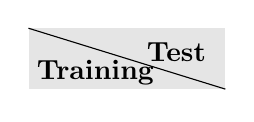
\begin{tikzpicture}[baseline=(B.base)]
  \node[inner sep=0pt,outer sep=0pt,
        minimum width=2.5cm,
        minimum height=2.2em,
        fill=mygray] (B) {};
  \draw (B.north west) -- (B.south east); % the diagonal
  \node[anchor=north east, xshift=-0.35em, yshift=-0.15em, font=\bfseries] at (B.north east) {Test};
  \node[anchor=south west, xshift=-0.05em, yshift=-0.20em, font=\bfseries] at (B.south west) {Training};
\end{tikzpicture}}%
}

\newcommand{\TwoRowGrayHeader}[2]{%
\multirow{2}{*}{%
\begin{tikzpicture}[baseline=(B.base)]
  \node[inner sep=0pt,outer sep=0pt,
        minimum width=#1,
        minimum height=2.2em,
        fill=mygray] (B) {};
  \node[font=\bfseries] at (B.center) {#2};
\end{tikzpicture}}%
}



\crefname{section}{\S}{\S\S}
\Crefname{section}{\S}{\S\S}


% Comment out this line in the camera-ready submission
\linenumbers

\urlstyle{same}

% the following package is optional:
%\usepackage{latexsym}

% See https://www.overleaf.com/learn/latex/theorems_and_proofs
% for a nice explanation of how to define new theorems, but keep
% in mind that the amsthm package is already included in this
% template and that you must *not* alter the styling.
\newtheorem{example}{Example}
\newtheorem{theorem}{Theorem}

% Following comment is from ijcai97-submit.tex:
% The preparation of these files was supported by Schlumberger Palo Alto
% Research, AT\&T Bell Laboratories, and Morgan Kaufmann Publishers.
% Shirley Jowell, of Morgan Kaufmann Publishers, and Peter F.
% Patel-Schneider, of AT\&T Bell Laboratories collaborated on their
% preparation.

% These instructions can be modified and used in other conferences as long
% as credit to the authors and supporting agencies is retained, this notice
% is not changed, and further modification or reuse is not restricted.
% Neither Shirley Jowell nor Peter F. Patel-Schneider can be listed as
% contacts for providing assistance without their prior permission.

% To use for other conferences, change references to files and the
% conference appropriate and use other authors, contacts, publishers, and
% organizations.
% Also change the deadline and address for returning papers and the length and
% page charge instructions.
% Put where the files are available in the appropriate places.


% PDF Info Is REQUIRED.

% Please leave this \pdfinfo block untouched both for the submission and
% Camera Ready Copy. Do not include Title and Author information in the pdfinfo section
\pdfinfo{
/TemplateVersion (IJCAI.2026.0)
}

\title{Instruction Granularity as Planning Width: Formalizing and\\Benchmarking for Vision-Language-Action Models}

% Single author syntax
\author{
    Author Name
    \affiliations
    Affiliation
    \emails
    email@example.com
}

% Multiple author syntax (remove the single-author syntax above and the \iffalse ... \fi here)
\iffalse
\author{
First Author$^1$
\and
Second Author$^2$\and
Third Author$^{2,3}$\And
Fourth Author$^4$\\
\affiliations
$^1$First Affiliation\\
$^2$Second Affiliation\\
$^3$Third Affiliation\\
$^4$Fourth Affiliation\\
\emails
\{first, second\}@example.com,
third@other.example.com,
fourth@example.com
}
\fi

\begin{document}

\maketitle

\begin{abstract}
    Real-world users provide instructions at varying levels of granularity, yet this remains an uncontrolled and unmeasured variable in Vision-Language-Action (VLA) research, leaving its impact unknown. 
    We formalize granularity as the \emph{planning demand} required to ground language into actions, and adapt \emph{rule width} from width-based planning to quantify this demand. To isolate and evaluate this variable, we introduce Mini-BEHAVIOR-Gran, extending all 20 complex tasks with: (i) a rule-set bank providing instruction variants across up to six granularity levels, and (ii) a dynamic instructor that delivers valid instructions at each step. Our analysis reveals a non-monotonic, U-shaped relationship between granularity and performance, with peaks at fine and coarse extremes. We demonstrate an asymmetry in generalization: models trained on coarse instructions transfer to fine ones, but not vice versa. Furthermore, we diagnose how coarse instructions can induce language-ignoring shortcuts due to high visual predictability, and identify mixed-granularity training regimens that best balance task performance with language grounding. Our findings establish instruction granularity as a fundamental dimension for diagnosing and improving multimodal alignment in VLAs.
\end{abstract}

% TODO : abstract Requite UPDATE to fit the latest observation
\section{Introduction}
\label{sec:introduction}

% Paragraph 1: Background 
% 快速总结现有VLA的背景和现状并且引出“粒度”这个维度的重要性。
When deploying Vision-Language-Action (VLA) models in the real world, a key challenge arises from natural variation in instruction granularity. Users may provide anything from highly precise commands to vague intentions \cite{clark1996using}. Handling instruction granularity is essential for human-agent interaction \cite{donalddesign2002}, yet current research faces two interrelated gaps that prevent a systematic answer.
% （修改说明：开篇点明核心问题后，立即用一句话总领下文，明确指出存在两个“缺口”，为下文的清晰分野定调。）

First, at the conceptual levels, the community has not yet reached a consensus on how to formally define or measure instruction granularity. 
A prevalent practice in hierarchical LLM agents \cite{DBLP:conf/wuwnet/Yang0H24} and recent VLA work \cite{DBLP:conf/corl/MyersZMFL24,DBLP:conf/icml/ShiIEKPVTWWFLDG25,zhong2025survey} is to operationalize granularity as the \emph{level of task decomposition}, i.e., whether an instruction specifies only the final goal or also enumerates subgoals. 
While intuitive, \emph{decomposition depth} is not a stable notion of granularity but dependent on the task structure: some tasks are intrinsically difficult yet do not admit meaningful hierarchical breakdowns due to \emph{interleaved subgoals} \cite{sussman1975computer}, whereas even simple tasks can be divided into many steps. In parallel, existing Natural Language Processing (NLP) studies of ``granularity'' typically focus on linguistic aspects, such as the \emph{level of detail} or \emph{discourse structure} of text \cite{dong-lapata-2018-coarse,huang-etal-2025-musc}, rather than adopting an embodied-agent-centric view to measure an instruction's \emph{informativeness} in terms of reducing the effort required to generate action plans. We instead depart from these proxies by defining instruction granularity as the \emph{planning demand} imposed by an instruction, i.e., how much internal search an agent must perform to ground the instruction into a concrete, executable plan. This framing explicitly decouples granularity from dedicated choices of task decomposition and yields a directly quantifiable measure within \emph{classical planning} frameworks, which is a better approach for analyzing and benchmarking VLA models. 

% （修改说明：这是第一个显性缺口。直接指出现有方法（任务分解）是什么，然后尖锐地批评其局限——“不任务无关”，并顺势引出我们主张的新视角（规划需求）。逻辑是：他们做了A，但A有问题，所以我们需要B。

Second, at the empirical level, variations of language granularity in existing VLA benchmarks is entangled with other factors. For example, benchmarks such as \textsc{BEHAVIOR-1K}, which focus on long-horizon activities, typically use abstract goal descriptions, whereas suites like \textsc{LIBERO}, which emphasize short-horizon robotic manipulation, adopt highly concrete commands \cite{DBLP:conf/cvpr/ShridharTGBHMZF20,DBLP:conf/corl/0002ZWGSMWLLSAH22,DBLP:conf/nips/LiuZGFLZS23,DBLP:conf/corl/LiHGMPWFLSKL0F024,DBLP:conf/cvpr/MuCCPLGLYZXLXDL25}. Therefore, it is difficult to disentangle a model's failure from either challenging perception, or complex low-level control as opposed to the impact of instruction granularity. In short, the field lacks a benchmark that holds tasks fixed while providing parallel instruction sets with rigorously controlled instruction granularity. To this end, the contributions of our paper are:

% （修改说明：这是第二个显性缺口。先陈述现状（不同基准有不同粒度），再指出其核心问题（粒度与任务属性纠缠），进而点明结果（无法独立研究）和缺失（缺乏受控基准）。逻辑清晰，与第一个缺口并列。）


\textbf{(1) A Domain-level Formalization:} We formalize instruction granularity as \emph{rule width}, a concept adapted from \emph{width-based planning} \cite{DBLP:conf/aaai/BonetFG19,DBLP:journals/jair/DrexlerSG24}. Intuitively, it measures how many state variables (i.e., \emph{features}) of the world state must be maintained \textbf{concurrently} when fulfilling an instruction (\Cref{sec:granularity_as_width}). This metric enables consistent comparison across tasks within the same domain, as it is defined over the shared domain-level feature set $\Phi$. More importantly, instruction granularity now reflects the \emph{informativeness} of an instruction when an embodied agent attempts to ground it into an action plan.

\textbf{(2) A Granularity-Controlled Benchmark:} We introduce \textsc{Mini-BEHAVIOR-Gran}, where each task is paired with multiple instruction variants spanning different granularity levels (\Cref{sec:benchmark}). It is the first-of-kind testbed that isolates instruction granularity as an independent variable, so as to enable controlled studies of its effects on VLA agents.


\textbf{(3) A Granularity-Centric View of Language Grounding:} We reveal a non-monotonic, U-shaped relationship between instruction granularity and VLA performance, identifying productive learning regimes at the extremes of Fine and Coarse instructions (\Cref{sec:experiments}). While prior work attributes ``language-ignoring'' primarily to statistical biases in training data, we provide a complementary granularity-centric perspective. We argue that instruction granularity is a structural driver of the trade-off between task success and language reliance. Through extensive evaluation across three action-decoding archetypes (Autoregressive, Diffusion, and Parallel), we demonstrate that coarse instructions can incentivize a bypass of linguistic grounding due to their higher predictability from visual state alone, whereas mixed-granularity training, particularly our proposed \emph{Axial-F} setting, best balances overall performance and language grounding.


% （修改说明：贡献部分严格、直接地回应了前面提出的两个缺口。贡献1针对Gap 1（概念与度量），贡献2针对Gap 2（评估基准），贡献3和4则是利用新工具产生的新发现和新解决方案。一一对应，逻辑闭环。）

Instruction granularity shapes the learning dynamics of VLA models trained on multimodal datasets. It introduces a dual risk: overly fine-grained instructions may degrade language into a mere identifier for specific state-action sequences, encouraging memorization rather than generalized understanding; conversely, overly coarse instructions can weaken language-action alignment, encouraging the model to exploit shortcuts in other data modalities---a risk that has been difficult to isolate and measure. Through our formalization and controlled benchmark, we provide the first systematic study of instruction granularity in VLAs, establishing it as a measurable dimension for future research on language grounding and multimodal alignment.
% TODO this part is a bit off, we are not really quantifying the trade-off. 

% TODO intro part need to rethink how to reflect the latest observation about attention sink

\section{Related Work}
\label{sec:related_work}

\textbf{Instruction Abstraction and Granularity.}
In this work, \emph{Instruction granularity} refers to the extent to which state and action constraints are explicitly specified versus left for the agent to infer when grounding language into actions.
This is distinct from, yet often conflated with the concept of \emph{linguistic abstraction}.
The term \emph{abstraction} is viewed as \emph{representational compression}---using a compact description to stand for multiple instances or executions. This definition is common in prior work of computational thinking \cite{Wing2010ComputationalTW,DBLP:journals/tacl/LachmyPMT22,DBLP:conf/iclr/ZhengMCCCLZ24}.
Importantly, granularity can vary independently of abstraction: ``tidy the room'' is coarse but non-abstract (it leaves the exact required actions underspecified, yet it lacks representational compression.), whereas ``repeat wiping until clean'' is relatively specific yet abstract (it prescribes an action but uses a loop condition to compress multiple executions).

While not framed as the term ``granularity'', we acknowledge that a rich body of work has focused on augmenting language specificity and its impact, for example through coarse-to-fine semantic parsing \cite{dong-lapata-2018-coarse,DBLP:conf/ijcai/LiLF020}.
Other work generates compositional instructions via constraint dropout and sub-task recombination \cite{huang-etal-2025-musc}, or construct counterfactual instructions to augment data diversity \cite{glossop2025castcounterfactuallabelsimprove}.

In embodied instruction following, varying instruction detail is often handled via a simple two-part decomposition: high-level plans are converted into sequences of low-level steps before being grounded into actions \cite{DBLP:conf/wuwnet/Yang0H24,DBLP:conf/icml/ShiIEKPVTWWFLDG25}. Most recent VLA works, however, operate with static language instructions \cite{ma2025surveyvisionlanguageactionmodelsembodied,li2025cogvla}. Some models like InstructVLA and ThinkAct explores having chain-of-thought reasoning steps before action decoding \cite{yang2025instructvlavisionlanguageactioninstructiontuning,huang2025thinkactvisionlanguageactionreasoningreinforced}. Despite this, quantitatively controlled studies on multi-level instruction granularity remain scarce in embodied AI domain.

\noindent\textbf{Language Sensitivity vs. Ignoring in VLA.} 
Recent studies present two seemingly contradictory findings. On one hand, VLA models appear sensitive to language variations, where semantically equivalent rephrasing of seen instructions leads to performance drops \cite{akula-etal-2022-alfred,karnik2025embodiedredteamingauditing}; this suggests a reliance on superficial word patterns. On the other hand, recent analyses identify a ``language-ignoring'' behavior, where models over-rely on visual context and bypass instructions entirely \cite{xing2025shortcut,fei2025liberoplus,xu2025seeingactpromptingspecify}. We provide a comprehensive granularity-centric view that reconciles these findings: instruction granularity modulates the balance between language sensitivity and ignoring, with overly coarse instructions leading to language-ignoring shortcuts.



\section{Rule Width as Instruction Granularity}
\label{sec:granularity_as_width}

\subsection{Running Example}
\label{subsec:running_example_init}
We first illustrate \emph{planning width} computation using a running example. \Cref{tab:task_width_scaling} shows the desired state progressions of a task where two shoes are cleaned using a rag, and the rag is placed on the floor afterwards. The key \textbf{environment dynamics} are: (1) the rag must be soaked before it can clean shoes, and (2) the sink must be turned on to soak the rag. We represent states using a set of task-relevant feature variables ($\Phi$): (i) boolean features $H_r$ (holding rag), $T_s$ (sink is turned on), $S_r$ (rag is soaked), $C_i$ (shoe $i$ is cleaned), $onfloor_r$ (rag is on the floor); and (ii) spatial features $p_r, p_s, p_f$ (distance to the rag, sink, and nearest uncleaned shoe, respectively).

\begin{table}[t]
\centering
\tiny
\begin{tabularx}{\columnwidth}{l X c}
\toprule
\textbf{State Progression} & \textbf{Concurrent Features Tracked (Sequence of Tuples)} & \textbf{Width} \\ \midrule
Initial State & $[\langle \rangle]$ & 0 \\
Navigate to rag & $[\langle p_r = X \rangle, \ldots, \langle p_r = 0 \rangle]$ & 1 \\
Pick up rag & $[\langle p_r = 0 \rangle, \langle H_r \rangle]$ & 1 \\
Navigate to sink & $[\langle H_r, p_s = X \rangle, \ldots, \langle H_r, p_s = 0 \rangle]$ & 2 \\
Turn on tap (sink) & $[\langle H_r, p_s = 0  \rangle,  \langle T_s \rangle]$ & 2 \\
Soak rag & $[\langle H_r, T_s, p_s = 0  \rangle, \langle S_r \rangle]$ & \textbf{3} \\
Navigate to Shoe 1 & $[\langle H_r, S_r, p_{f1} \downarrow \rangle, \ldots,] $ & \textbf{3} \\
Clean Shoe 1 & $[\langle H_r, S_r, p_{f1} = 0 \rangle, \langle C_1 \rangle]$ & 3 \\
Navigate to Shoe 2 & $[\langle H_r, S_r, C_1, p_{f2} \downarrow \rangle, \ldots ]$ & \textbf{4} \\
Clean Shoe 2 & $[\langle H_r, S_r, C_1  , p_{f2} = 0 \rangle, \langle C_1, C_2   \rangle]$ & 4 \\
Put rag on floor & $[\langle C_1, C_2, H_r \rangle, \ldots, \langle C_1, C_2, \text{onfloor}_r \rangle]$ & 3 \\ \bottomrule
\end{tabularx}
\caption{State progression and width for the ``Cleaning $k$ Shoes'' ($k=2$). Width scales as $w = k+2$.}
\label{tab:task_width_scaling}
\end{table}

First, approaching the rag is a navigation-only segment: the desired state progression is to decrease the distance feature $p_r$ until $p_r=0$. Thus, the width is 1 as only a single feature needs to be tracked. In this environment dynamics, $p_r=0$ enables the state transition to $H_r$. Thus, the rag can be obtained at $p_r=0$ and the width remains $1$. Subsequently, $H_r$ must be maintained while progressing to next states, resulting in a width of $2$. The rag becoming soaked requires simultaneous maintenance of three features, i.e., at the sink ($p_s=0$), holding the rag ($H_r$), and having the sink turned on ($T_s$), which yields a width of $3$. After soaking, $C_1$ can be obtained by tracking $H_r$, $S_r$, and $p_f$, giving width 3. The subtlety arises when cleaning the second shoe: one has to track the same features as before, plus maintaining the cleanliness of the first shoe ($C_1$), which increases the width to $4$. 


\paragraph{Why no action model?}
Agents' action sets constrain how state transitions are executed, but \emph{width} focuses on state-level feature dependencies induced by the environment dynamics. Different agents (e.g., a rover vs. a drone) may have different action spaces to achieve the same feature change, so emphasizing state progressions promotes generalization of width-based concepts across different embodiments.


% NOTE: In this section, we need to transition from the intuitive concept of "planning demand" to a rigorous, quantifiable metric. Since we are adapting Rule Width from classical planning (Bonet et al., 2019), the structure should mirror a formal derivation: starting from a standard planning domain and ending with a metric that can be applied to natural language instructions via their symbolic grounding.

The impact of \emph{instruction granularity} on VLA behavior remains underexplored largely because the field lacks a \textbf{formal, quantifiable, cross-task} measure of granularity. The most common heuristic, \emph{decomposition depth} \cite{DBLP:conf/corl/MyersZMFL24,DBLP:conf/icml/ShiIEKPVTWWFLDG25}, is unstable as discussed in \Cref{sec:introduction}. To bridge this gap, we formalize \emph{instruction granularity} as \emph{planning demand}---the internal search required to ground an instruction into an executable plan. This perspective captures the intuitive difference between fine- and coarse-grained instructions: fine-grained instructions provide a ``breadcrumb trail''  that narrows the search, whereas coarse instructions leave a much larger solution space to be explored to reach a state that fulfills the instruction.

We operationalize planning demand using \textbf{rule width} ($w$), adapting the notion of \emph{planning width} from classical planning \cite{DBLP:conf/ecai/LipovetzkyG12} and its extension to \emph{policy sketches} \cite{DBLP:conf/aaai/BonetG21,DBLP:conf/aips/DrexlerSG22,DBLP:journals/jair/DrexlerSG24}. We first introduce the underlying task representation, then model instructions as sets of ``if-then'' rules that decompose tasks, and finally define rule width as a measure of instruction granularity for these rule sets.

\subsection{Symbolic Task Representation}

While VLAs operate on raw multimodal observations, we adopt a symbolic, relational state abstraction. Many embodied benchmarks provide such structured representations---object properties and relations---that can be expressed as \emph{fluents} to form symbolic state or goal conditions \cite{shridhar2020alfred,DBLP:conf/corl/LiHGMPWFLSKL0F024}. Formally , we consider a classical planning problem $P = \langle \mathcal{F}, \mathcal{A}, I, G \rangle$, where $\mathcal{F}$ is a set of fluents, $\mathcal{A}$ a set of actions, $I$ the initial state, and $G$ the goal. 

To bridge raw states and high-level instructions, we define a set of \textbf{features} $\Phi = \{\phi_1, \ldots, \phi_n\}$, where $\phi_i$ is a Boolean or integer-valued function over state space $S$. These features serve as domain-level abstractions that capture task-relevant aspects of the environment. Thus, each $s$ is associated with a \textbf{feature valuation vector} $\phi(s) = \left(\phi_1(s), \ldots, \phi_n(s)\right)$.

\subsection{Instructions as Rule Sets $\mathcal{R}$}

To study instruction granularity in a controlled manner, we formalize each instruction a symbolic interpretation as a set of ``if-then'' rules $\mathcal R = \{r_1,\ldots, r_m\}$ defined over the feature space $\Phi$, This rule-based representation does not aim to capture the full expressiveness of natural language; instead, it distills the constraint/goal structure that governs the computational cost incurred by a symbolic search algorithm (i.e., planning demand). Specifically, each $r_i$ is of the form $C_{r_i} \mapsto E_{r_i}$:
\begin{itemize}
    \item $C_{r_i}$ (the \emph{condition}) is a conjunction of feature constraints. For a Boolean feature $p$, a constraint is $p$ or $\lnot p$; for a numerical feature $n$, it is $n = 0$ or $n > 0$.
    \item $E_{r_i}$ (the \emph{effect}) is a conjunction of feature changes. For a Boolean feature $p$, an effect is $p$, $\lnot p$, or $p?$ (allowing any change); for a numerical feature $n$, it is $n\downarrow$ (decrease), $n\uparrow$ (increase), or $n?$ (any change).
\end{itemize}
These forms capture the core semantics of the instructions we study. A rule $r_i$ is \textbf{fulfilled} by a state sequence $(s, \dots, s')$ if $\phi(s) \models C_i$ and the pair $(\phi(s), \phi(s'))$ satisfies the changes in $E_i$ (e.g., $\forall (n \downarrow) \in E_{r_i}, \phi_n(s') < \phi_n(s)$) while keeping unmentioned features constant (i.e., $\phi_j(s') = \phi_j(s)$ for $j \notin E_i$).

In our experiments, all natural-language instructions presented to the VLA agent are designed such that their symbolic interpretations, i.e., the rule sets $\mathcal R$ over features $\Phi$, are \textbf{well-formed} (i.e., goal-separating and terminating) and it is guaranteed that at least one \textbf{sound} and \textbf{closed} \cite{DBLP:conf/aaai/BonetG21} policy exists on all benchmark instances, so rule-following ensures dead-end-free reachability. This rule-based framing explicitly exposes the latent subgoal structure, enabling controlled variation of how much structural guidance the instruction provides.

\subsection{Rule Width as a Granularity Measure}
\label{subsec:rule_width_granularity}
% (规则宽度作为粒度度量) 核心贡献部分。首先基于宽度理论，定义单条规则的宽度。然后，定义整个指令（即规则集）的宽度为其所有规则宽度的最大值。最后，论证该度量如何对应指令粒度：低宽度=细粒度（提供详细子目标），高宽度=粗粒度（留下更多并发规划需求）。
We quantify instruction granularity through \emph{rule width} ($w$), a metric that captures the peak concurrent planning demand required to ground language into action. The intuition is rooted in the mechanism of \textbf{Iterated Width (IW)} search \cite{DBLP:conf/ecai/LipovetzkyG12}. IW($k$) is a novelty-guided breadth-first search algorithm that retains a state only if it makes some previously unseen combination of $k$ feature values true. Thus, if a rule $r_i$ has width $w(r_i)=2$, then reaching its effect $E_i$ from a state $s$ with  $\phi(s) \models C_i$ can be fulfilled by tracking at most two features concurrently (to be made
precise with a running example in \Cref{subsec:running_example}); consequently, IW($2$) is guaranteed to find a shortest-path plan to fulfill $r_i$ if one exists. $w(r_i)=0$ is a special case where $r_i$ can be fulfilled in a single step.

The granularity of an instruction (i.e., rule set $\mathcal R$) is then defined as the maximum width across its rules:
\begin{equation}
    w(\mathcal R) = \max_{r_i \in \mathcal R} w(r_i).
\end{equation}

\subsection{Running Example Continued}
\label{subsec:running_example}
% (贯穿实例) 使用一个具体任务（例如您提到的“铺设木地板”），完整演示上述过程：任务的目标、定义的特征、为不同粒度设计的规则集，以及计算出的规则宽度。用此例直观说明“宽度”如何作为调节指令粒度的旋钮。

\begin{figure*}[t]
    \centering
    
\includegraphics[width=0.92\linewidth]{figures/experiment_illu.pdf}
    \caption{\textsc{Mini-BEHAVIOR-Gran} Experimental Pipeline. We evaluate the impact of instruction granularity across three VLA action-decoding strategies. During inference time, an Oracle Instructor evaluates the current world state to decide available rule set $\mathcal R_a$ and active rule $r_t$. A rule-based natural language instruction $l_t$ is generated accordingly. The process iterates until completion or max steps.}
    \label{fig:experiment_illu}
\end{figure*}


\begin{figure}
    \centering
    
\includegraphics[width=\linewidth]{figures/running_examples.pdf}
    \caption{(Left) factoring $r_1$ into $r_{1a}$-$r_{1c}$ reduces the planning complexity that the agent must handle internally. More explicit linguistic guidance makes the mapping to action easier to learn. (Right) the long-horizon trajectory for the coarse rule ($\pi_{r_1}$, red) is broken into shorter segments by the finer-grained instructions.}
    \label{fig:running_example}
\end{figure}




We continue to demonstrate three instruction sets, each representing a different width level, with two variants visualized in \Cref{fig:running_example}. We also append a \textbf{counting feature} in $\Phi$ to track the number of uncleaned shoes, denoted as $N_f$.

\paragraph{Coarse-Grained Instruction ($w(\mathcal R) = 3$ )} This instruction states only the high-level rules and their desired ordering, leaving the internal structure of each sub-task implicit:
\begin{itemize}
    \item $r_1 : \{N_f > 0\} \mapsto \{N_f \downarrow\}$ (clean a shoe; $w=3$)
    \item $r_2 : \{N_f = 0, \neg onfloor_{r}\} \mapsto \{onfloor_{r}\}$ (put the rag on the floor after cleaning all shoes; $w=1$)
\end{itemize}

% (Two-column figure spanning the top of the page)Panel A: Admissible Chains. A comparison table of "Working Memory" requirements. Shows how $w=3$ requires a 3-feature tuple, while $w=1$ breaks the task into single-feature "stepping stones."Panel B: Feature Tracking Profile. A plot showing the tuple size (active feature tracking) over the task duration. $w=3$ shows a high, sustained peak; $w=1$ shows a low, consistent baseline.Panel C: The Grounding Gap. A conceptual diagram visualizing the "Informational Void" where the agent must rely on learned biases rather than explicit instructions.

\paragraph{Middle-Grained Instruction ($w(\mathcal R) = 2$ )} This variant decomposes $r_1$ to explicitly state the \emph{soaking} process:
\begin{itemize}
    \item $r_{1a} : \{\neg H_r\} \mapsto \{H_r\}$ (pick up the rag; $w = 1$)
    \item $r_{1b} : \{H_r, \neg S_r \} \mapsto \{S_r, H_r?\}$ (soak the rag; $w = 2$)
    \item $r_{1c} : \{N_f > 0, S_r \} \mapsto \{N_f \downarrow\}$ (clean; $w = 2$)
    \item $r_2 : \{N_f = 0, \neg onfloor_{r}\} \mapsto \{onfloor_{r}\}$ (put the rag on the floor; $w = 1$)
\end{itemize}
This rule set is well-formed: it is goal-terminating via $r_2$, and the rules are sequentially reachable, meaning the successor state of any fulfilled rule (that is not the goal) satisfies the condition of at least one rule in $\mathcal{R}$. The set is also robust to perturbations: if an agent drops the rag after soaking it ($\neg H_r$), the rule set remains applicable by reverting to $r_{1a}$ to reacquire the rag before proceeding to the cleaning task ($r_{1c}$). 

\noindent \textbf{Width Analysis of $r_{1b}$}: From an algorithmic perspective, the width $w(r)$ is the smallest $k$ such that IW($k$) solves $r$. Consider $r_{1b}$ (soaking the rag): if the instruction were expressed as a isolated transition $\{\neg S_r\} \mapsto \{S_r\}$, an agent would need to concurrently coordinate three features: holding the rag ($H_r$), reaching the sink ($p_s = 0$), and toggling the sink ($T_s$). However, because $r_{1b}$'s precondition requires $H_r$ to be established (via $r_{1a}$), and given that IW search explores states in breadth-first order, any plan that undoes an established feature is necessarily longer than one that preserves it and is subsequently pruned as suboptimal. Hence, the agent can treat $H_r$ as a maintained rather than an actively tracked feature. This reduces the concurrent feature tracking to $\langle T_s, p_s = 0 \rangle$, yielding $w(r_{1b})= 2$. Although the VLA agent does not perform explicit IW search, this width serves as a rigorous proxy for the inherent planning burden imposed by the instruction.



\paragraph{Fine-grained Instruction ($w=1$)} This variant further decomposes the task into six rules where each transition addresses at most one feature change. The task is fully serialized into three stages: preparation ($r_1: \{\neg H_r\} \mapsto \{H_r\}$; $r_2: \{\neg T_s\} \mapsto \{T_s\}$; $r_3: \{H_r, T_s, \neg S_r\} \mapsto \{S_r\}$); cleaning ($r_4: \{N_f > 0, \neg H_r, S_r\} \mapsto \{H_r\}$; $r_5: \{N_f > 0, H_r, S_r\} \mapsto \{N_f \downarrow\}$); and storage ($r_6: \{N_f = 0, \neg onfloor_{r}\} \mapsto \{onfloor_{r}\}$). The higher rule count and denser preconditions is the explicit indicators of increased instruction granularity. This shift displaces the planning complexity to explicit structural textual guidance. The resulting training data exhibits a more direct language-to-action mapping, thereby reducing the grounding gap that VLA agents must learn to bridge.

To communicate these rules to VLA agents, we translate each rule into a natural-language sentence via a template-based generator. These templates verbalize the features within each rule; e.g., $\{\hlA{$H_r$}, \hlB{$\neg S_r$}\} \mapsto \{\hlC{$S_r$}\}$ is realized as ``If you are \hlA{holding the rag} but \hlB{the rag is not yet soaked}, \hlC{soak the rag}.'' This construction preserves the granularity differences defined by the rule width. Additional language prompt examples are provided in \Cref{app_sec:prompt_examples}.


\section{Mini-BEHAVIOR-Gran Benchmark}
\label{sec:benchmark}
% Step 1: 首先介绍我们想要什么的benchmark: 要能够更isolate instruction granularity 的影响，然后visual perception difficulty 和 low level action control complexity 都要简单（从而避免confound）
% 然后我们看一下之前mini behavior 自己是怎么justify自己的：
% We present a new simplified benchmark, Mini-BEHAVIOR, that provides the benefits of simple
% benchmarks for fast prototyping and training, while keeping the most relevant problem structure and
% the characteristics from the task-level decision-making challenge in BEHAVIOR: the long-horizon,
% heterogenousness of the activities, and the multi-object, multi-state, high variability of household
% environments. Mini-BEHAVIOR re-defines BEHAVIOR tasks in a novel 3D Gridworld environment
% with support for procedural generation for potentially infinite variants of each task.

% Step 2: 因此我们选择在mini behavior的基础上进行扩展。然后之说我们在appendix 上有更详细的justification. Details on why these environments are \textbf{preferred over other test benchmarks} are provided in \Cref{app_sec:ant_defense_test_env}.

To disentangle the influence of instruction granularity in VLA performance, we seek an environment that (1) retains long-horizon and heterogeneous activities so that instruction guidance meaningfully modulates the planning demand, while (2) simplifies perception and low-level control to avoid confounding factors. As such, we use \textsc{Mini-BEHAVIOR} \cite{jin2023minibehavior} as our testbed. Detailed justification for our choice over other environments is provided in \Cref{app_sec:ant_defense_test_env}.

% Step 3: 要不要给一个表写上是哪些20 tasks 然后我提供的granularity levels for each task 有哪些（我感觉可以放在appendix里）
% Step 4: 介绍offline dataset construction 是用了 BFWS planner 来 generate plans corresponding to the rule sets. 然而在inference time, 我们使用oracle instructor 来 generate filter and select valid rule to generate instruction by accessing the internal state of the environment to get current feature valuations $\phi(s)$ 然后 check which rule conditions are satisfied (需要formula), 然或说 \Cref{fig:experiment_illu} 进行说明。

We introduce \textsc{Mini-BEHAVIOR-Gran}, the first VLA benchmark specifically designed to enable a controlled study and formal quantification of instruction granularity via \emph{rule width}. Specifically, we define a shared, domain-level feature set $\Phi$ that captures task-relevant attributes across all 20 complex household tasks on top of the symbolic state abstraction from the original benchmark. For each task, we design rule sets with varying widths (up to six levels). We verify that all rule sets are well-formed and solvable. We utilize an Oracle Instructor to deliver instructions during inference. This ensures that any observed performance drops are strictly attributable to the model's inability to ground specific granularity levels, rather than stochastic variations in instruction quality or applicability that would confound our cross-granularity analysis (see \Cref{fig:experiment_illu} right panel). At each time $t$, it evaluates the current feature vector $\phi(s_t)$, identifies the set of available rules $\mathcal{R}_{\text{a}} = \{r \in \mathcal{R} \mid \phi(s_t) \models C_r\}$. We sample an active rule $r_t \in \mathcal{R}_{\text{a}}$ and it is then processed by a template-based translator to generate a natural language instruction $l_t$, to match the VLA model's input format. $l_t$ is paired with the current observation $v_t$ and fed into the VLA model to predict action chunk $(a_t, ..., a_{t+k}) \sim \pi_{\text{vla}}(\cdot \mid v_t, l_t)$.


% Step 5: 上价值，need to highlight that our finding can Transfer beyond Mini-BEHAVIOR，我门的feature set 是specific to household domains, 但是不是specific to mini-behavior. 

% \textsc{Mini-BEHAVIOR-Gran} serves as a first-of-its-kind testbed for studying instruction granularity in VLA. By anchoring to an environment-wide feature abstraction $\Phi$, our formalization remains cross-task available, thereby supporting an open-ended set of activities defined over $\Phi$. Moreover, new features can be appended to support additional domains while keeping existing ones intact, allowing extension to other embodied environments that support symbolic state abstraction.


\section{Experiments}
\label{sec:experiments}
% **话术：** “由于这是首个系统性研究指令粒度的 Benchmark，我们的实验重点在于揭示 **Instruction Granularity ($w$)** 与 **Learning Burden** 之间的本质联系。我们不追求在多个异构 Benchmark 上刷榜，而是在一个受控的环境中探索指令粒度对 VLA 的影响函数。”
\subsection{Experimental Setup}
\paragraph{Task Suite \& Training.} We use \textsc{Mini-BEHAVIOR-Gran}, which contains 20 complex tasks sharing the same feature set $\Phi$. We further classify instruction granularity into three \emph{relative} classes of \emph{Fine (F)}, \emph{Medium (M)}, and \emph{Coarse (C)} via per-task quantile binning. In most cases, this mapping corresponds to $w=0$ for Fine, $w=1$ for Medium, and $w \ge 2$ for Coarse. We evaluate seven training settings: (1) \textbf{Pure F/M/C} ($1\!:\!0\!:\!0$): trains exclusively on one granularity class; (2) \textbf{Centroid} ($1\!:\!1\!:\!1$): uniformly sample from all three classes; (3) \textbf{Axial F/M/C} ($3\!:\!1\!:\!1$): emphasizes one class with some exposure to the rest classes. Our dataset provides 50 training and 10 evaluation instances per task, each paired with reference trajectories for every granularity level generated by \textsc{BFWS} width-based planner from Lipovetzky and Geffner \shortcite{DBLP:conf/aaai/LipovetzkyG17} (see \Cref{app_sec:minibehavior_gran_details} for details).

% \paragraph{Relative Instruction Binning.} A significant challenge in evaluating instruction granularity is that different tasks possess inherently different structural depths; for instance, opening_packages may only support a maximum width of $w=1$, whereas cleaning_the_kitchen extends to $w=5$. To maintain a balanced evaluation across this heterogeneous suite, we implement a per-task quantile-based binning strategy. For each domain, we sort the available symbolic widths and partition them into three relative levels: Fine (Low), Medium, and Coarse (High). In cases with limited width availability, we apply a priority-fill heuristic to ensure every task contributes to all three experimental categories. This normalization allows us to observe universal performance trends across the complexity spectrum, independent of the absolute planning width of any specific task.

\paragraph{Action-Decoding Archetypes.} The primary architectural difference among latest VLA models lies in their action-decoding strategies \cite{zhong2025survey}. Hence, we employ a unified VLM backbone but vary three representative action-decoding strategies (see \Cref{fig:experiment_illu} left panel): (1) \textbf{Autoregressive} (AR), exampled by RT-2 \cite{DBLP:conf/corl/ZitkovichYXXXXW23}, OpenVLA \cite{DBLP:conf/corl/KimPKXB0RFSVKBT24} and others \cite{DBLP:journals/tmlr/ReedZPCNBGSKSEBREHCHVBF22,DBLP:conf/icml/HuangYMLLW0ZJ024,DBLP:conf/icra/ONeillRMGPLPGMJ24} that predict actions sequentially via causal attention; (2) \textbf{(Discrete) Diffusion}, which uses diffusion process for action chunk prediction \cite{pmlr-v305-black25a,bjorck2025gr00t,shukor2025smolvla}. We employ discrete diffusion \cite{liang2025discrete} for compatibility with the discrete action space of our testbed; (3) \textbf{Parallel Decoding}, utilizing bidirectional attention for single-pass action prediction to improve throughput, as demonstrated by OpenVLA-OFT \cite{kim2025fine}, PD-VLA \cite{DBLP:conf/iros/SongCDZZZGLWWML25} and other variants \cite{yin2025deepthinkvla,wang2025bitvla,xiao2025ava}. Details on model hyperparameters, hardwares and training schedules are in \Cref{app_sec:implementation_details}.

\paragraph{Research Questions.} We address the following questions:

\noindent\textbf{(Q1)} \textbf{Granularity Trade-offs.} How does instruction granularity impact Success Rate \textbf{(SR)} on within splits?

\noindent\textbf{(Q2)} \textbf{Generalization.} Can VLA agents trained on certain granularities generalize to other unseen granularities? 

\noindent\textbf{(Q3)} \textbf{Failure Dynamics.} When failing, does the agent get stuck (stagnation) or undo achieved progress (regression)?

% 就是因为 coarse instruction会好点 出现了U-shape。
% 然后这个其实值得研究。 所以你就进一步看 到底是它拿到了visual shortcut 还是说 因为语言太模糊了， 只能更多的依赖grounding

\subsection{Main Results}

We first answer \textbf{(Q1)}, short answers as follows:

\begin{figure*}[t]
    \centering
    \begin{minipage}[t]{0.33\textwidth}
        \centering
        
\includegraphics[width=\linewidth]{figures/q1_main.pdf}
        \captionof{figure}{In-Distribution (matched train/test) SR across granularities (i.e., train Fine$\rightarrow$test Fine, etc). A U-shaped trend appears.}
        \label{fig:q1_learning_curves}
    \end{minipage}\hfill
    \begin{minipage}[t]{0.66\textwidth}
        \centering
        
\includegraphics[width=\linewidth]{figures/q3_training_setting_on_sr_across_width.pdf}
        \captionof{figure}{The x-axis are test instruction width, and the y-axis are training setup. Transfer is asymmetric: train coarse $\rightarrow$ test fine works, but train fine $\rightarrow$ test coarse does not. Mixed-granularity training improves generalization. \emph{Axial-C} training setting performs best overall.}
        \label{fig:q3_cross_granularity}
    \end{minipage}
\end{figure*}

\begin{figure*}[t]
    \centering
    \begin{minipage}[t]{0.30\textwidth}
        \centering
        
\includegraphics[width=\linewidth]{figures/q1_rule_call_dist.pdf}
        \captionof{figure}{Rule call distribution across instruction granularities. \# of rule calls decreases with coarser instructions. It decouples instruction length from width.}
        \label{fig:q1_rule_call_dist}
    \end{minipage}\hfill
    \begin{minipage}[t]{0.30\textwidth}
        \centering
        
\includegraphics[width=0.9\linewidth]{figures/q1_width_vs_task_horizon_heatmap.pdf}
        \captionof{figure}{Impact of width and horizon on SR. SR decays with task horizon; larger instruction width imposes an additional burden even when horizon is fixed.}
        \label{fig:q1_width_vs_task_horizon_heatmap}
    \end{minipage}\hfill
    \begin{minipage}[t]{0.32\textwidth}
        \centering
        
\includegraphics[width=\linewidth]{figures/q4_failure_type_extreme_task_example.pdf}
        \captionof{figure}{Low-width but long task horizon (e.g., laying woods) tends to cause regression, while high-width tasks tend to stagnate. These contribute to the failure of planning.}
        \label{fig:q4_failure_modes}
    \end{minipage}
\end{figure*}


\textbf{(A1)} \emph{VLA performance follows a non-monotonic \emph{U-shape}, peaking at the Fine and Coarse extremes.}

To establish a performance baseline, we first evaluate the models under matched granularity, where training and testing occur on the same instruction class ($F \to F$, $M \to M$, $C \to C$). As shown in \Cref{fig:q1_learning_curves}, all three action-decoding archetypes demonstrate a non-monotonic U-shaped discovery. Note that all instructions are generated via a unified template-based translator that directly verbalizes symbolic rule sets, ensuring uniform vocabulary, syntax, and phrasing across granularity levels and isolating rule width as the causal factor. We interpret this U-shaped curve as follows. When instructions provide a step-by-step mapping to actions (i.e., $w=0$), the learning burden is minimal, as the agent can directly follow instructions with little reasoning or planning effort. At the coarse end ($w \ge 2$), agents are motivated to develop internal planning skills to ground coarse instructions into actions. Importantly, since each coarse instruction maps to a broader set of visual and action patterns, it helps develop more robust and generalizable language grounding by providing more diverse training data. In contrast, medium instructions ($w\!=\!1$) occupy a sub-optimal grounding regime. They are too sparse to provide a direct language-to-action mapping, yet not coarse enough to foster internal planning skills, thereby resulting in the performance decline.

From a width-based planning perspective, the U-shaped pattern surprises because coarser instructions should monotonically increase planning demands, making learning progressively harder. Yet, a common confounding factor is instruction sequence length (i.e., the number of rule calls required to complete a task), which also impacts SR due to error accumulation. Note that our evaluation uses the same underlying task set across granularities, and thus the reference atomic action sequence length is held constant. The only entangled factor is thus the rule call count. As shown in \Cref{fig:q1_rule_call_dist}, coarser instructions require fewer rule calls to accomplish the same task, as each instruction maps to a longer action sequence. The medium granularity operates at a moderate number of rule calls. This decouples instruction sequence length from instruction width and confirms the U-shape cannot be attributed to medium-granularity tasks requiring excessively longer instruction sequences or rule calls.

To further decouple the effects of instruction width and sequence length on VLA performance, we analyze \Cref{fig:q1_width_vs_task_horizon_heatmap}, obtained by \emph{Centroid} setting as it has balanced exposure to all granularities. The heatmap provides empirical evidence that, for a fixed number of rule calls, SR decreases as instruction width increases. This demonstrates that the width metric, originally developed for symbolic planning, is a meaningful proxy for the difficulty faced by learning-based VLA agents.

Next, we evaluates cross-granularity generalization, where models are trained on one instruction granularity and evaluated on another. Results are summarized in below:

\textbf{(A2)} \emph{Language grounding is asymmetric: models trained on coarse texts generalize to detailed ones, but not vice versa.}

\Cref{fig:q3_cross_granularity} reveals a clear asymmetry: models trained on coarse instructions generalize well to fine ones, demonstrating robust language grounding that abstracts away from granularity. Conversely, models trained on fine instructions do not generalize to coarse ones, implying a form of grounding that overfits to step-by-step specification. Mixed-granularity training mitigates this issue, with the coarse-weighted \emph{Axial-C} variant yielding the best generalization overall.

\begin{figure*}[t]
    \centering
    \begin{minipage}[t]{0.41\textwidth}
        \centering
        
\includegraphics[width=\linewidth]{figures/q5_sr_diff_by_training_setup.pdf}
        \captionof{figure}{Both mixed and coarse-only training ``generalize'' better in novel instruction settings (smaller SR gap).}
        \label{fig:sr_diff_by_training_setup}
    \end{minipage}\hfill
    \begin{minipage}[t]{0.54\textwidth}
        \centering
        
\includegraphics[width=\linewidth]{figures/q6_compare_baseline_models_attention_dist.pdf}
        \captionof{figure}{Attention from action tokens. Self-attention dominates, followed by vision; No clear trend across granularity levels.}
        \label{fig:attention_distribution_baseline_models}
    \end{minipage}
\end{figure*}

% \begin{figure*}[t]
% \centering
%     
\includegraphics[width=0.7\linewidth]{figures/q6_attention_distribution_across_model_types_vs_sent_enc.pdf}
%     \captionof{figure}{Action-token attention across three decoding architectures ($\pm$ sentence encoding). Self-attention dominates, followed by vision; \textit{Discrete diffusion} attends more to language than the others. Sentence encoding reduces vision and self-attention, but induce attention sink.}
%     \label{fig:q5_attention_distribution_across_model_types_vs_sent_enc}
% \end{figure*}


For \textbf{(Q3)}, the failure mode is dependent on task structure:

\textbf{(A3)} \emph{Low-width but long-horizon tasks tend to cause regression, while high-width tasks tend to stagnate.}

We interpret these failure modes through the lens of width-based planning (see \Cref{fig:q4_failure_modes}). In high-regression tasks, which often require manipulating multiple objects toward a collective goal, agents frequently exhibit subgoal serialization failures. In these settings, the model fails to maintain satisfied fluents over time, cycling back to earlier states. Conversely, stagnation in high-width tasks (e.g., making tea) reflects a width-planning bottleneck: as simultaneous feature dependencies increase ($w \ge 4$), agents struggle to track multiple simultaneous feature dependencies to enable a valid state progression. More analysis is in \Cref{app_sec:additional_experimental_results}.


\section{Dilemma of Coarse Instruction Training}
\label{sec:more_analysis_on_coarse_instruction_training}

Our analyses in \textbf{(Q1)} and \textbf{(Q3)} suggest a practical advantage for training with coarse instructions: models maintain strong in-distribution performance while generalizing effectively to unseen, finer-grained instructions. To further evaluate this generalization capability, we test robustness to more extreme instruction variations: providing only a static goal description (fixed for the entire episode, akin to the \textsc{LIBERO} testbed \cite{DBLP:conf/nips/LiuZGFLZS23}) and providing no instruction at all.

Results are shown in \Cref{fig:sr_diff_by_training_setup}. Mixed-granularity training, particularly the \emph{Axial-C} variant, achieves the highest SR when presented with the unseen static-goal descriptions. More strikingly, when the language input is entirely absent, \emph{Axial-C} maintains a non-trivial SR of 21\%. This raises a fundamental question: does the success of coarse instruction training stem from improved generalization via robust language grounding, or from ``language ignoring'', where the policy becomes invariant to language inputs?

\paragraph{Quantifying Language Ignoring.}
``Language ignoring'' is a phenomenon recently identified in VLA training, where agents appear to over-rely on visual patterns, making their policies invariant to language input \cite{xing2025shortcut,fei2025liberoplus}. A standard metric for this is $\Delta\mathrm{SR} = \mathrm{SR}{\text{w/ lang}} - \mathrm{SR}{\text{w/o lang}}$, where a smaller gap indicates stronger ignoring. Our data reveals a trend: models trained purely on coarse instructions (\emph{Pure-C}) exhibit a smaller $\Delta\mathrm{SR}$ (20.0\%) than those trained on fine instructions (\emph{Pure-F}), suggesting coarser training may induce greater language ignoring. 

\paragraph{Attention Analysis.}
To probe the model's internal reliance on language more directly, we analyze the attention distribution from action tokens to the vision, language, and self-modalities (see \Cref{fig:attention_distribution_baseline_models}). Contrary to a simple visual-shortcut hypothesis, we find no clear trend of decreasing attention to the language modality as instruction granularity coarsens. Across all training regimes, self-attention receives the largest share, followed by vision, with language consistently receiving the smallest portion. Notably, autoregressive models attend least to language, which could explain their lower overall SR in \Cref{fig:q1_learning_curves}. 

\paragraph{Why Coarse Instructions Encourage Language Ignoring?}
Xu et. al. \shortcite{xu2025seeingactpromptingspecify} posit a causal mechanism: if the language instruction $l$ is highly predictable from visual context $v$ (i.e., large $P(l \mid v)$), a multimodal model may learn to bypass language processing to save computational energy. This aligns with our benchmark, where expert trajectories are fixed but described at varying granularities: consider a surjective mapping $f$ from a fine-grained label space $L_{\text{fine}} = {l_1, \dots, l_n}$ to a coarser one $L_{\text{coarse}} = {c_1, \dots, c_m}$ with $m < n$. The conditional probability for a coarse label aggregates over its constituent fine labels: $P(c_j | v) = \sum_{l_i \in f^{-1}(c_j)} P(l_i | v)$. Since the same total probability mass is distributed over fewer coarse categories, the average $P(c_j | v)$ is higher. According to the theory, this increased predictability could encourage language ignoring for coarsely-trained models.

Mixed-granularity training mitigates this effect by increasing the diversity of the language space $L$ seen during training, which lowers the average $P(l \mid v)$. We thus see all mixed-granularity models exhibit larger $\Delta\mathrm{SR}$ gaps than their pure counterparts, indicating reduced language ignoring. Among these, the fine-weighted mixture \emph{Axial-F} emerges as a particularly balanced choice, achieving a success rate comparable to \emph{Axial-C} while maintaining a substantially larger $\Delta\mathrm{SR}$. 

Our analysis provides a complementary perspective on the language ignoring phenomenon, demonstrating its variation across instruction granularities, a factor not explored in prior work. The trade-off between final performance and language reliance highlights an open challenge in VLA design: how to structure training for both robust generalization and faithful language grounding.

\section{Conclusion and Future Work}
\label{sec:conclusion}
% 在论文的局限性部分，主动、诚恳地讨论上述部分问题（如环境的简化、动态指导的理想化），并阐述未来如何在本工作基础上进行扩展研究（如在更复杂环境中验证、研究稀疏指令下的规划）。这能展现您思考的全面性，并化解审稿人的部分质疑。
This work formalizes and systematically studies how instruction granularity impacts the performance and generalization of VLA agents. Our controlled analysis shows that VLA performance is highly sensitive to granularity, exhibiting a non-monotonic U-shaped relationship that suggests real-world systems may benefit from deliberate instruction granularity design. We provide a granularity-centric diagnosis of the ``language ignoring'' phenomenon, linking it to instruction predictability and identifying mixed-granularity training as an effective mitigation strategy.

\paragraph{Future Work.}
Several promising directions follow. First, moving beyond symbolic, grid-based domains to estimate \emph{planning width} in complex, continuous environments would greatly enhance generalizability. This requires developing methods to approximate \emph{width} from ambiguous observations and diverse instruction formats. Second, to enable this, a key challenge is the automatic derivation of relevant feature sets. Future work could develop learnable feature modules that dynamically extract or construct planning-relevant state abstractions directly from multimodal inputs (pixels, knowledge bases, or language descriptions), reducing reliance on hand-designed symbolic predicates and bridging the gap between vectorized data and structured planning models.

\paragraph{Use of LLM Statement} An LLM was used only for polishing language; the scientific content is entirely original.


% POTENTIAL REBUTTAL We acknowledge the reviewer’s concern regarding evaluation on a single benchmark. However, in planning and symbolic reasoning research—where precise control over task structure, state abstraction, and instruction semantics is essential—it is standard practice to conduct in-depth analysis within a well-designed, controlled environment (e.g., MiniGrid, BabyAI, PDDL-based domains, or custom grid worlds in [ICAPS, NeurIPS, ICLR] works). Our goal is not broad empirical coverage, but rather a disentangled study of how instruction granularity affects VLA behavior under formally defined conditions. The design of Mini-BEHAVIOR-Gran enables this level of control, which would be impossible in off-the-shelf benchmarks. We believe this focused approach aligns with methodological norms in the planning and neuro-symbolic communities.

% \printbibliography[segment=0]
\bibliographystyle{named_short}
\bibliography{ijcai26}

\onecolumn
\appendix
% \newrefsegment %% <== increases the segment number (0 by default)
% Start of appendices customization
\titleformat{\section}
  {\normalfont\Large\bfseries\centering}{\thesection}{1em}{}

\begin{center}
    \textbf{\huge Technical Appendix}
\end{center}
\section*{Appendix Table of Contents}
\begin{enumerate}
    \item \textbf{Anticipatory defense on the choice of test environments and metrics} (\Cref{app_subsec:app_sec:ant_defense_test_env}) \\
    Justification for chosen test environments and evaluation metrics.
\end{enumerate}

\section{Anticipatory defense on the choice of test environments and metrics}
\label{app_sec:ant_defense_test_env}

% 主动承认并界定研究范围：明确指出，本工作的首要目标是机理研究，而非追求极致的现实仿真。Mini-BEHAVIOR在保留家庭任务的长视距、多对象、状态依赖等高层级决策复杂性的同时，主动剥离了低层级感知与控制的噪音。这使我们能够将模型失败更清晰地归因于语言grounding和规划问题，而非纹理识别或连续运动控制。

% 使用“先理解，再扩展”的研究范式论证：引用经典研究范式——先在受控的简化环境中理解核心机理，再将验证过的假设推广到更复杂的场景。可以说明，我们的形式化方法（规则宽度）是任务和平台无关的，未来可以在更复杂的仿真器中复用同一套指令生成与控制框架。

% 对比优势：简要对比指出，在iGibson等高级仿真器中，难以程序化地生成海量、精确对应不同规则宽度的指令-轨迹对，且渲染和物理计算成本过高，不利于进行需要大量实验迭代的消融研究。

In this work, we selected Mini-BEHAVIOR as our testbed. This choice is motivated by several key considerations aligned with our research objectives. Our research objective is not to solve the full stack of robotic embodiment (which includes perception, continuous control, and physics), but specifically to isolate and analyze the impact of instruction granularity on language grounding and long-horizon planning.

Therefore, high-fidelity simulators (e.g., iGibson \citep{li2022igibson}, BEHAVIOR-1K \citep{DBLP:conf/corl/0002ZWGSMWLLSAH22}) introduce significant noise through complex texture rendering and continuous motor control. While realistic, these factors act as confounders. When an agent fails in such environments, it is often difficult to attribute the failure to a lack of linguistic understanding (granularity issues) or a failure in low-level execution (e.g., grasping physics or occlusion). Mini-BEHAVIOR retains the high-level decision complexity of household tasks—long horizons, multi-object interactions, and state dependencies—while abstracting away low-level sensorimotor noise.

In the perspective of fast prototyping and iterative experimentation, we have to also consider the rendering and physics simulation costs. Mini-BEHAVIOR's grid-based discrete control and simplified visual representation allow for rapid data generation and model training. 

Another consideration is the diversity of the task structures so that we can systematically vary instruction granularity across a wide range of scenarios. As such, Crafter \citep{hafner2021crafter}, which focuses on survival in a single domain, lacks the diverse task structures needed to obtain robust insights about instruction granularity. 

Table \ref{tab:env_comparison} provides a detailed comparison of Mini-BEHAVIOR against other prominent benchmarks, highlighting why they were less suitable for this specific investigation.

\begin{table*}[t]
\small
\centering
\caption{Comparison of Embodied AI Environments regarding their suitability for studying Instruction Granularity.}
\label{tab:env_comparison}
\begin{tabular}{@{}l>{\raggedright\arraybackslash}p{1.4cm}c>{\raggedright\arraybackslash}p{1.5cm}>{\raggedright\arraybackslash}p{1.7cm}>{\raggedright\arraybackslash}p{4.9cm}@{}}
\toprule
\textbf{Environment} & \textbf{Control} & \textbf{Horizon} & \textbf{Visuals} & \textbf{Symbolic Abstraction} & \textbf{Limitation} \\
\midrule
\textbf{Mini-BEHAVIOR}(*) & Discrete & Long & Grid & \textbf{Support} & \textbf{Ideal balance:} Supports symbolic state abstraction; diverse task suite; removes control noise while retaining logic complexity. \\
\textbf{Crafter} & Discrete & Long & Cartoon & Partial & Single task suite (survival); partially observable (memory heavy); few object types. \\
\textbf{Meta-World} & Continuous & Short & 3D & No & Continuous control; no symbolic abstraction; focus on multi-task RL/manipulation, not long-horizon planning. \\
\textbf{LIBERO} & Continuous & Short & 3D & No & Robotic arm focus; continuous control; no symbolic abstraction; VLA success rate already saturated (tasks relatively easy). \\
\textbf{RoboTwin 2.0} & Continuous & Short & 3D & No & Continuous control; no symbolic abstraction; dual-arm manipulation focus; hard to segment expert trajectories and construct granular instructions. \\
\textbf{CALVIN} & Continuous & Medium & 3D & No & Hard to design instruction granularity due to continuous action space (though provides diverse language); confounds planning with control difficulties. \\
\textbf{ALFRED} & Discrete & Long & 3D Photo & Support & 3D partially observable; poor infrastructure support for VLA training; high rendering cost. \\
\textbf{iGibson / BEHAVIOR-1K} & Continuous & Long & 3D Photo & Partial & Good for long-horizon tasks, but 3D realistic vision context becomes a confounder. \\
\bottomrule
\end{tabular}%
\end{table*}

\section{Symbolic Representation of the Embodied Task}
\label{app_sec:classical_prob_def}


We formalize the Mini-BEHAVIOR environment as a deterministic grid-based symbolic world. This allows us to represent the challenge as a classical planning problem $\mathcal{P} = \langle \mathcal{F}, \mathcal{A}, s_0, G \rangle$, where:
\begin{itemize}[leftmargin=*]
    \item $\mathcal{F}$ is a finite set of propositional fluents representing the state variables of the environment (e.g., object locations, states like \textit{cooked} or \textit{open}).
    \item $\mathcal{A}$ is a finite set of actions available to the agent.
    \item $s_0 \subseteq \mathcal{F}$ is the initial state configuration.
    \item $G \subseteq \mathcal{F}$ is the goal condition that must be satisfied.
\end{itemize}
A state $s \in \mathcal{S}$ is defined as a truth valuation over $\mathcal{F}$, with the state space $\mathcal{S} \subseteq 2^\mathcal{F}$ encompassing all valid combinations of fluent truth values.

\section{Details of \textsc{Mini-BEHAVIOR} Environment}
\label{app_sec:minibehavior_details}

To operationalize our formalism, we developed a \textbf{Universal PDDL Domain Model} (available at \url{minibehavior_gran_domain_model.pddl} in the codebase) capable of supporting all 20 household tasks without modification. This unified model comprises over 1,000 lines of PDDL 2.1 definitions and is fully compatible with the LAMA planner. We highly recommend checking the codebase for the complete domain model.

\paragraph{Search Space Characteristics}
\begin{table}[H]
    \centering
    \small
    \caption{Planning complexity in typical tasks.}
    \label{tab:planning_complexity}
    \begin{tabular}{@{}lc@{}}
        \toprule
        \textbf{Metric} & \textbf{Typical Range} \\
        \midrule
        Objects & 15--40 \\
        Grid Locations & 20--60 \\
        Ground Actions & $10^3$--$10^5$ \\
        Plan Length & 50--200 primitive actions \\
        Planning Time (LAMA) & 0.5--300+ seconds \\
        \bottomrule
    \end{tabular}
\end{table}

\section{Details of \textsc{Mini-BEHAVIOR-Gran} Extension}
\label{app_sec:minibehavior_gran_details}

\textsc{Mini-BEHAVIOR} provides the foundational task skeletons, which we extend in \textsc{Mini-BEHAVIOR-Gran} to support multi-granularity instruction generation. A core component of this extension is the definition of a symbolic feature set used to generate rule-based policy sketches.


\subsection{Feature Categories}

The environment defines two primary categories of features: Boolean State Features and Quantitative Features.

\subsubsection{Boolean State Features}
These features evaluate whether a specific object instance satisfies a predicate. They require grounding (binding to specific object instances, e.g., \texttt{rag-01}).

\begin{table}[t]
\centering
\caption{Boolean State Features}
\label{tab:bool_features}
\resizebox{\columnwidth}{!}{%
\begin{tabular}{l|l|l}
\hline
\textbf{Feature} & \textbf{Applicable Objects} & \textbf{Semantics} \\ \hline
\texttt{Holding} & All Items & Is the agent holding the specified object? \\
\texttt{isOpened} & Cabinets, Drawers, Doors & Is the container/door open? \\
\texttt{isToggled} & Sinks, Stoves, Switches & Is the appliance turned on? \\
\texttt{isSoaked} & Rags, Sponges & Is the cleaning tool wet? \\
\texttt{isCleaned} & Shoes, Dishes, Floor & Is the object free of stains? \\
\texttt{isDustFree} & Furniture, Surfaces & Is the object free of dust? \\ \hline
\end{tabular}%
}
\end{table}

\subsubsection{Quantitative and Spatial Features}
These features capture distances, counts, and spatial relationships. Crucially, they support temporal comparison allowing conditions such as ``distance decreased'' or ``count dropped to zero.''

\begin{itemize}[leftmargin=*]
\item \textbf{\texttt{DistanceToNearest(type, condition)}}: Measures the Manhattan distance from the agent to the nearest object of a specific type.
\begin{itemize}[leftmargin=*]
\item \textit{Conditions:} \texttt{=0} (adjacent), \texttt{>0}, \texttt{increase}, \texttt{decrease}, \texttt{change}.
\end{itemize}
\item \textbf{\texttt{Count(type, condition, function)}}: Counts the number of objects of a specific type that satisfy a filter function.
\begin{itemize}
\item \textit{Conditions:} \texttt{=0}, \texttt{>0}, \texttt{increase}, \texttt{decrease}.
\end{itemize}
\end{itemize}

\subsection{Count Functions}
A diverse set of counting functions is implemented to support complex logical conditions (e.g., ``all shoes are clean'' is equivalent to \emph{count\_not\_cleaned == 0}).

\begin{table}[t]
\centering
\caption{Available Count Functions for Rule Definitions}
\label{tab:count_funcs}
\resizebox{\columnwidth}{!}{%
\begin{tabular}{l|l}
\hline
\textbf{Category} & \textbf{Function Description} \\ \hline
\textbf{State-Based} & \texttt{count\_not\_cleaned}: Objects that are currently stained. \\
& \texttt{count\_not\_soaked}: Cleaning tools that are dry. \\
& \texttt{count\_not\_toggled}: Appliances that are turned off. \\
& \texttt{count\_closed}: Containers/doors that are closed. \\
& \texttt{count\_not\_sliced}: Food items that require slicing. \\ \hline
\textbf{Spatial} & \texttt{count\_not\_onfloor}: Objects not placed on the floor layer. \\
& \texttt{count\_isolated}: Objects with no neighbors of the same type. \\
& \texttt{count\_not\_inside\_target}: Objects not contained within a specific furniture. \\
& \texttt{count\_not\_ontop}: Objects not placed on top of a specific surface. \\
& \texttt{count\_not\_near\_target}: Objects not within 1 step of a target type. \\ \hline
\textbf{Task-Specific} & \texttt{count\_incomplete\_salad}: Plates lacking necessary ingredients. \\
& \texttt{count\_not\_complete\_tables}: Tables lacking specific setups (e.g., candles). \\ \hline
\end{tabular}%
}
\end{table}

% \subsection{Activation and Verification Mechanism of Oracle Instructor}
% To support relative conditions (e.g., \textit{``distance decreased''}), features utilize a two-step verification process:
% \begin{enumerate}
% \item \textbf{Precondition Activation:} The feature state is recorded before an action sequence.
% \item \textbf{Effect Verification:} The feature is checked after execution against the stored value.
% \end{enumerate}
% This mechanism is essential for defining granular instructions that describe \textit{progress} (e.g., ``move closer to the sink'') rather than just static states.


\subsection{Reference Plan Generation and Task Complexity Analysis} \label{app_sec:ref_plan_gen}

While the original \textsc{Mini-BEHAVIOR} framework provides the high-level skeletons for household activities, it does not provide reference plans by default. Thus, we utilize the \textsc{BFWS} (Best-First Width Search) classical planner to generate reference plans for all 20 tasks in \textsc{Mini-BEHAVIOR-Gran}. These reference plans serve as the ground truth for our agents and allow us to quantitatively categorize the complexity of each task.

\begin{figure*}[t]
    \centering
    
\includegraphics[width=\textwidth]{figures/plan_steps_distribution_boxplot.png}
    \caption{Distribution of reference plan steps required for tasks in \textsc{Mini-BEHAVIOR-Gran} obtained by \textsc{BWFS} classical planner.}
\end{figure*}


% ===== Fused Benchmark Task Spec Table (ID + OOD) with Goal Description =====

\begin{table*}[ht]
\small
\vspace{3mm}
\centering
\label{table:benchmark_task_spec}\scalebox{0.90}{{
\begin{tabular}{>{\centering\arraybackslash}p{4.9cm}||c|c|p{8.4cm}|c}
\toprule[0.4mm]
\cellcolor{mygray}\textbf{Task} & \cellcolor{mygray}\textbf{Split} & \cellcolor{mygray}\textbf{Class} & \cellcolor{mygray}\textbf{Goal Description} & \cellcolor{mygray}\textbf{Mean Steps} \\
\hline \hline
opening\_packages & ID & \cellcolor{green!20}\textbf{short} & Open every package. & 10.2 \\
installing\_a\_printer & ID & \cellcolor{green!20}\textbf{short} & Place a printer on a table and turn it on. & 10.6 \\
laying\_wood\_floors & ID & \cellcolor{green!20}\textbf{short} & Lay every plywood sheet on the floor, each touching at least one other sheet. & 15.9 \\
moving\_boxes\_to\_storage & ID & \cellcolor{green!20}\textbf{short} & Place every carton inside a shelf. & 36.3 \\
cleaning\_a\_car & ID & \cellcolor{green!20}\textbf{short} & Make at least one car dust-free. Place a rag and soap together inside a bucket. & 62.6 \\
throwing\_away\_leftovers & ID & \cellcolor{yellow!25}\textbf{middle} & Throw away every hamburger by placing it in a trash can. & 68.3 \\
organizing\_file\_cabinet & ID & \cellcolor{yellow!25}\textbf{middle} & Put a marker on a table and file every folder and document in a cabinet. & 75.5 \\
making\_tea & ID & \cellcolor{yellow!25}\textbf{middle} & Slice a lemon. Put a teapot on an activated stove. Keep a soaked teabag with the teapot. & 78.7 \\
sorting\_books & ID & \cellcolor{yellow!25}\textbf{middle} & Place every book and every hardback on a shelf. & 78.8 \\
collect\_misplaced\_items & ID & \cellcolor{yellow!25}\textbf{middle} & Place all gym shoes, necklaces, notebooks, and socks on a table. & 90.7 \\
thawing\_frozen\_food & ID & \cellcolor{yellow!25}\textbf{middle} & Place a date label next to a fish. Put every fish next to a sink. Set an olive next to a sink. & 101.7 \\
boxing\_books\_up\_for\_storage & ID & \cellcolor{blue!15}\textbf{long} & Place every book inside a box. & 134.4 \\
storing\_food & ID & \cellcolor{blue!15}\textbf{long} & Store every cookable item inside a cabinet. & 144.6 \\
preparing\_salad & ID & \cellcolor{blue!15}\textbf{long} & Slice all apples and tomatoes; place them on plates. Put every radish and lettuce on plates. Ensure each plate holds at least one cookable item. & 146.7 \\
putting\_away\_dishes\_after\_cleaning & ID & \cellcolor{blue!15}\textbf{long} & Put every plate inside a cabinet. & 147.7 \\
cleaning\_up\_the\_kitchen\_only & ID & \cellcolor{blue!15}\textbf{long} & Put every blender on a countertop. Refrigerate all apples and casseroles. Keep soap next to a sink. Make plates unstained and cabinets dust-free. Place each rag either beside or inside the sink. Store plates and vegetable oil in different cabinets. & 161.0 \\
setting\_up\_candles & ID & \cellcolor{blue!15}\textbf{long} & On every table, place three distinct candles on top. & 165.2 \\
\hline
cleaning\_shoes & OOD & \cellcolor{green!20}\textbf{short} & Leave a towel on the floor and make sure every shoe is unstained and dust-free. & 54.2 \\
watering\_houseplants & OOD & \cellcolor{yellow!25}\textbf{middle} & Water every potted plant until it is soaked. & 79.4 \\
washing\_pots\_and\_pans & OOD & \cellcolor{blue!15}\textbf{long} & Clean every teapot, kettle, and pan so they're unstained, then store each inside a cabinet. & 149.5 \\
\bottomrule[0.4mm]
\end{tabular}}}
\caption{Classification of tasks in \textsc{Mini-BEHAVIOR-Gran} based on the median number of plan steps, as determined by the \textsc{BWFS} planner. Tasks are categorized into short, middle, and long classes to reflect varying planning complexity based on plan length.}
\label{table:benchmark_class_based_on_plan_steps}
\end{table*}

Detailed statistics regarding the specific rule sets used for instruction generation and the resulting natural language statistics are discussed in the next section.


\section{Rule Set and Natural Language Prompt Examples For Different Tasks}
\label{app_sec:prompt_examples}

We present the rank 0 rule set for 10 over 20 household tasks in the Mini-BEHAVIOR-Gran environment. For other levels, please refer to the codebase at \url{mini-behavior-gran/mini_behavior/utils/policy_sketch/}. 

\subsection{Task 1: Laying Wood Floors}

\textbf{Features:}
\begin{itemize}[noitemsep]
    \item $H$: holding an isolated wood (plywood)
    \item $p$: distance to the nearest isolated wood
    \item $t$: distance to an arbitrary (non-held) wood we'll place next to
    \item $n$: number of isolated woods
\end{itemize}

\resizebox{\columnwidth}{!}{$
\begin{aligned}
\{\neg H, p>0, n >0\} &\mapsto \{p \downarrow, t?\} && \text{; move close to isolated wood} \\
\{\neg H, p=0, n >0\} &\mapsto \{H\} && \text{; pick up isolated wood when reachable} \\
\{H, t>0, n >0\} &\mapsto \{t\downarrow\} && \text{; move to some wood location} \\
\{H, n >0, t=0\} &\mapsto \{H?, n \downarrow, p?\} && \text{; drop the isolated wood next to other wood}
\end{aligned}
$}
\subsection{Task 2: Preparing Salad}

\textbf{Features:}
\begin{itemize}[noitemsep]
    \item $H_n$: holding a not-sliceable food
    \item $H_s$: holding a sliceable food
    \item $H_k$: holding a slicer
    \item $U$: number of sliceable food that is not sliced yet
    \item $d_p$: distance to the selected incomplete plate $p$
    \item $d_n, d_s$: distances to nearest not-sliceable / sliceable
    \item $k$: distance to a slicer (knife)
    \item $B$: selected plate $p$ complete bottom salad
    \item $n$: number of incomplete plates
    \item $nn$: number of plates that do not have bottom salad yet
\end{itemize}

\resizebox{\columnwidth}{!}{$
\noindent\textit{Acquire slicer:}
\begin{aligned}
\{U>0 , \neg H_k, k>0\} &\mapsto \{k \downarrow\} && \text{; move to slicer} \\
\{U>0 , \neg H_k, k=0\} &\mapsto \{H_k\} && \text{; hold a slicer} \\
\{U>0 , H_k, d_s > 0\} &\mapsto \{d_s \downarrow\} && \text{; move to sliceable food} \\
\{U>0 , H_k, d_s = 0\} &\mapsto \{U \downarrow, \neg H_k \} && \text{; cut sliceable food} \\
\{U=0 , H_k\} &\mapsto \{\neg H_k\} && \text{; put down slicer}
\end{aligned}
$}
\resizebox{\columnwidth}{!}{$
\noindent\textit{Place bottom salad:}
\begin{aligned}
\{n>0, U=0, nn>0, \neg B, \neg H_n, d_n>0\} &\mapsto \{d_n \downarrow\} \\
\{n>0, U=0,nn>0, \neg B, \neg H_n, d_n=0\} &\mapsto \{H_n\} \\
\{n>0, U=0,nn>0, \neg B, H_n, d_p>0\} &\mapsto \{d_p\downarrow\} \\
\{n>0, U=0, nn>0, \neg B, H_n, d_p=0\} &\mapsto \{B, nn \downarrow, \neg H_n\}
\end{aligned}
$}

\resizebox{\columnwidth}{!}{$
\noindent\textit{Handle sliceable salad:}
\begin{aligned}
\{nn=0, n>0, U=0 , \neg H_s, d_s>0\} &\mapsto \{d_s \downarrow\} && \text{; move to sliceable food} \\
\{nn=0, n>0, U=0 , \neg H_s, d_s=0\} &\mapsto \{H_s\} && \text{; pick up sliceable food} \\
\{nn=0, n>0, U=0 , H_s, d_p>0\} &\mapsto \{d_p \downarrow\} && \text{; move to the plate} \\
\{nn=0, n>0, U=0 , H_s, d_p=0\} &\mapsto \{n \downarrow, \neg H_s\} && \text{; put down sliced food}
\end{aligned}
$}

\subsection{Task 3: Cleaning Up the Kitchen Only}

\textbf{Features:}
\begin{itemize}[noitemsep]
    \item \textit{Holding flags:} $H_b$ (blender), $H_f$ (food), $H_s$ (soap), $H_r$ (rag), $H_p$ (plate), $H_o$ (vegetable oil)
    \item \textit{Distances:} $d_{ct}$ (countertop), $d_{fr}$ (fridge), $d_{si}$ (sink), $d_{c1}$ (cabinet for plate), $d_{c2}$ (cabinet for oil), $d_x$ (to object $x$)
    \item \textit{State booleans:} $\text{Open}(c)$, $\text{Tog}(s)$, $\text{Soaked}$, $\text{DustFree}(c)$, $\text{Clean}(p)$, $\text{OilIn}(c_2)$, $\text{Diff}$
    \item \textit{Counters:} $N_b$ (blenders not on countertop), $N_a$ (apples not in fridge), $N_{cas}$ (casseroles not in fridge), $N_s$ (soaps not next to sink), $N_{cab}$ (cabinets not dusted), $N_r$ (rags not next to sink), $N_{p\_clean}$ (plates not clean), $N_{oil}$ (oil not in cabinet), $N_{p\_store}$ (plates not stored), $N_{close}$ (closed furniture)
\end{itemize}

\resizebox{\columnwidth}{!}{$
\noindent\textit{Open Cabinet and Fridge:}
\begin{aligned}
\{N_{close} > 0, d_c>0\} &\mapsto \{d_c\downarrow\} && \text{; move toward closed furniture} \\
\{N_{close} > 0, d_c = 0\} &\mapsto \{N_{close}\downarrow\}
\end{aligned}
$}

\resizebox{\columnwidth}{!}{$
\noindent\textit{Oil placement:}
\begin{aligned}
\{N_{close} = 0,\neg H_o, d_{oil}>0\} &\mapsto \{d_{oil}\downarrow\} && \text{; approach oil} \\
\{N_{close} = 0,\neg H_o, d_{oil}=0\} &\mapsto \{H_o\} && \text{; pick up oil} \\
\{N_{close} = 0, H_o, N_{oil} > 0, d_{c2}>0\} &\mapsto \{d_{c2}\downarrow\} && \text{; go to cabinet } c_2 \\
\{N_{close} = 0, H_o, N_{oil} > 0, d_{c2} = 0\} &\mapsto \{N_{oil}\downarrow, \neg H_o\} && \text{; place oil in } c_2
\end{aligned}
$}

\resizebox{\columnwidth}{!}{$
\noindent\textit{Plate cleaning:}
\begin{aligned}
\{\neg \text{Tog}(s), d_{si}>0\} &\mapsto \{d_{si}\downarrow\} && \text{; toggle sink on} \\
\{\neg \text{Tog}(s), d_{si}=0\} &\mapsto \{\text{Tog}(s)\} \\
\{\neg H_r, d_{rag}>0\} &\mapsto \{d_{rag}\downarrow\} && \text{; get rag} \\
\{\neg H_r, d_{rag}=0\} &\mapsto \{H_r\} \\
\{H_r, \neg \text{Soaked}, d_{si}>0\} &\mapsto \{d_{si}\downarrow\} && \text{; soak rag} \\
\{H_r, \neg \text{Soaked}, d_{si}=0\} &\mapsto \{\text{Soaked}\} \\
\{H_r, \text{Soaked}, N_{p\_clean}>0, d_{plate}>0\} &\mapsto \{d_{plate}\downarrow\} \\
\{H_r, \text{Soaked}, N_{p\_clean}>0, d_{plate}=0\} &\mapsto \{N_{p\_clean}\downarrow, d_{plate}?\}
\end{aligned}
$}
\resizebox{\columnwidth}{!}{$
\noindent\textit{Plate placement distinct from oil:}
\begin{aligned}
\{N_{close} =0 , N_{oil}=0, N_{p\_clean} =0 ,\neg H_p, N_{p\_store}>0, d_{plate}>0\} &\mapsto \{d_{plate}\downarrow\} \\
\{N_{close} =0 , N_{oil}=0, N_{p\_clean} =0 , \neg H_p, N_{p\_store}>0, d_{plate}=0\} &\mapsto \{H_p\} \\
\{N_{close} =0 , N_{oil}=0, N_{p\_clean} =0 , H_p, N_{p\_store}>0, d_{c1}>0\} &\mapsto \{d_{c1}\downarrow\} \\
\{N_{close} =0 , N_{oil}=0, N_{p\_clean} =0 , H_p, N_{p\_store}>0, d_{c1}=0\} &\mapsto \{N_{p\_store}\downarrow, \neg H_p\}
\end{aligned}
$}

\resizebox{\columnwidth}{!}{$
\noindent\textit{Blender to countertop:}
\begin{aligned}
\{N_b > 0, \neg H_b, d_{blender}>0\} &\mapsto \{d_{blender}\downarrow\} \\
\{N_b > 0, \neg H_b, d_{blender}=0\} &\mapsto \{H_b\} \\
\{H_b, N_b>0, d_{ct}>0\} &\mapsto \{d_{ct}\downarrow\} \\
\{H_b, N_b>0, d_{ct}=0\} &\mapsto \{N_b\downarrow, \neg H_b\}
\end{aligned}
$}

\resizebox{\columnwidth}{!}{$
\noindent\textit{Apple to fridge:}
\begin{aligned}
\{N_{close} =0,\neg H_f, d_{apple}>0\} &\mapsto \{d_{apple}\downarrow\} \\
\{N_{close} =0,\neg H_f, d_{apple}=0\} &\mapsto \{H_f\} \\
\{N_{close} =0,H_f, N_a>0, d_{fr}>0\} &\mapsto \{d_{fr}\downarrow\} \\
\{N_{close} =0,H_f, N_a>0, d_{fr}=0\} &\mapsto \{N_a\downarrow, \neg H_f\}
\end{aligned}
$}

\resizebox{\columnwidth}{!}{$
\noindent\textit{Casserole to fridge:}
\begin{aligned}
\{N_{close} =0 ,\neg H_f, d_{casserole}>0\} &\mapsto \{d_{casserole}\downarrow\} \\
\{N_{close} =0 ,\neg H_f, d_{casserole}=0\} &\mapsto \{H_f\} \\
\{N_{close} =0 ,H_f, N_{cas}>0, d_{fr}>0\} &\mapsto \{d_{fr}\downarrow\} \\
\{N_{close} =0 ,H_f, N_{cas}>0, d_{fr}=0\} &\mapsto \{N_{cas}\downarrow, \neg H_f\}
\end{aligned}
$}

\resizebox{\columnwidth}{!}{$
\noindent\textit{Cabinet dusting:}
\begin{aligned}
\{\neg H_r, d_{rag}>0\} &\mapsto \{d_{rag}\downarrow\} && \text{; get rag} \\
\{\neg H_r, d_{rag}=0\} &\mapsto \{H_r\} \\
\{H_r, N_{cab}>0, d_c>0\} &\mapsto \{d_c\downarrow\} && \text{; clean cabinet} \\
\{H_r, N_{cab}>0, d_c=0\} &\mapsto \{N_{cab}\downarrow, \neg H_r\}
\end{aligned}
$}

\resizebox{\columnwidth}{!}{$
\noindent\textit{Rag near/inside sink:}
\begin{aligned}
\{N_{cab} = 0, N_{p\_clean} = 0,\neg H_r, d_{rag}>0\} &\mapsto \{d_{rag}\downarrow\} \\
\{N_{cab} = 0, N_{p\_clean} = 0,\neg H_r, d_{rag}=0\} &\mapsto \{H_r\} \\
\{N_{cab} = 0, N_{p\_clean} = 0,H_r, N_r>0, d_{si}>0\} &\mapsto \{d_{si}\downarrow\} \\
\{N_{cab} = 0, N_{p\_clean} = 0,H_r, N_r>0, d_{si}=0\} &\mapsto \{N_r\downarrow, \neg H_r\}
\end{aligned}
$}

\resizebox{\columnwidth}{!}{$
\noindent\textit{Soap next to sink:}
\begin{aligned}
\{N_{cab} = 0, N_{p\_clean} = 0,\neg H_s, d_{soap}>0\} &\mapsto \{d_{soap}\downarrow\} \\
\{N_{cab} = 0, N_{p\_clean} = 0,\neg H_s, d_{soap}=0\} &\mapsto \{H_s\} \\
\{N_{cab} = 0, N_{p\_clean} = 0,H_s, N_s>0, d_{si}>0\} &\mapsto \{d_{si}\downarrow\} \\
\{N_{cab} = 0, N_{p\_clean} = 0,H_s, N_s>0, d_{si}=0\} &\mapsto \{N_s\downarrow, \neg H_s\}
\end{aligned}
$}

\subsection{Task 4: Organizing File Cabinet}

\textbf{Features:}
\begin{itemize}[noitemsep]
    \item $H_m$: holding a marker
    \item $H_f$: holding a folder
    \item $H_d$: holding a document
    \item $p_m$: distance to the nearest marker
    \item $p_f$: distance to the nearest folder
    \item $p_d$: distance to the nearest document
    \item $p_t$: distance to a table
    \item $p_c$: distance to a valid cabinet target
    \item $N_m$: number of markers not on a table
    \item $N_f$: number of folders not in a cabinet
    \item $N_d$: number of documents not in a cabinet
    \item $N_o$: number of closed cabinets
\end{itemize}

\resizebox{\columnwidth}{!}{$
\noindent\textit{Opening Cabinet:}
\begin{aligned}
\{N_o > 0, p_c > 0\} &\mapsto \{p_c \downarrow\} && \text{; move toward a closed cabinet} \\
\{N_o > 0, p_c = 0\} &\mapsto \{N_o \downarrow\} && \text{; open the cabinet when reachable}
\end{aligned}
$}
\resizebox{\columnwidth}{!}{$
\noindent\textit{Marker task:}
\begin{aligned}
\{N_m > 0, \neg H_m, p_m > 0\} &\mapsto \{p_m \downarrow, p_t ?\} && \text{; move toward the nearest marker} \\
\{N_m > 0, \neg H_m, p_m = 0\} &\mapsto \{H_m, p_t ?\} && \text{; pick up the marker when reachable} \\
\{N_m > 0, H_m, p_t > 0\} &\mapsto \{p_t \downarrow\} && \text{; move toward a table} \\
\{N_m > 0, H_m, p_t = 0\} &\mapsto \{N_m \downarrow, \neg H_m, p_m ?\} && \text{; put marker on table}
\end{aligned}
$}
\resizebox{\columnwidth}{!}{$
\noindent\textit{Folder task:}
\begin{aligned}
\{N_f > 0, N_o = 0, \neg H_f, p_f > 0\} &\mapsto \{p_f \downarrow, p_c ?\} \\
\{N_f > 0, N_o = 0, \neg H_f, p_f = 0\} &\mapsto \{H_f, p_c ?\} \\
\{N_f > 0, N_o = 0, H_f, p_c > 0\} &\mapsto \{p_c \downarrow\} \\
\{N_f > 0, N_o = 0, H_f, p_c = 0\} &\mapsto \{N_f \downarrow, \neg H_f, p_f ?\}
\end{aligned}
$}
\resizebox{\columnwidth}{!}{$
\noindent\textit{Document task:}
\begin{aligned}
\{N_d > 0, N_o = 0, \neg H_d, p_d > 0\} &\mapsto \{p_d \downarrow, p_c ?\} \\
\{N_d > 0, N_o = 0, \neg H_d, p_d = 0\} &\mapsto \{H_d, p_c ?\} \\
\{N_d > 0, N_o = 0, H_d, p_c > 0\} &\mapsto \{p_c \downarrow\} \\
\{N_d > 0, N_o = 0, H_d, p_c = 0\} &\mapsto \{N_d \downarrow, \neg H_d, p_d ?\}
\end{aligned}
$}

\subsection{Task 5: Thawing Frozen Food}

\textbf{Features:}
\begin{itemize}[noitemsep]
    \item $H_{fish}$: holding a fish
    \item $H_{olive}$: holding an olive
    \item $H_{date}$: holding a date
    \item $p_{fish}$: distance to the nearest fish
    \item $p_{olive}$: distance to the nearest olive
    \item $p_{date}$: distance to the nearest date
    \item $p_{sink}$: distance to a sink
    \item $N_{fish}$: number of fish not next to a sink
    \item $N_{olive}$: number of olives not next to a sink
    \item $N_{date}$: number of dates not next to a fish
\end{itemize}

\resizebox{\columnwidth}{!}{$
\noindent\textit{Fish Task:}
\begin{aligned}
\{\neg H_{fish}, p_{fish} > 0\} &\mapsto \{p_{fish} \downarrow\} \\
\{\neg H_{fish}, p_{fish} = 0\} &\mapsto \{H_{fish}\} \\
\{H_{fish}, p_{sink} > 0\} &\mapsto \{p_{sink} \downarrow\} \\
\{H_{fish}, p_{sink} = 0\} &\mapsto \{N_{fish} \downarrow, \neg H_{fish}, p_{fish} ?\}
\end{aligned}
$}

\resizebox{\columnwidth}{!}{$
\noindent\textit{Olive Task:}
\begin{aligned}
\{\neg H_{olive}, p_{olive} > 0\} &\mapsto \{p_{olive} \downarrow\} \\
\{\neg H_{olive}, p_{olive} = 0\} &\mapsto \{H_{olive}\} \\
\{H_{olive}, p_{sink} > 0\} &\mapsto \{p_{sink} \downarrow\} \\
\{H_{olive}, p_{sink} = 0\} &\mapsto \{N_{olive} \downarrow, \neg H_{olive}, p_{olive} ?\}
\end{aligned}
$}

\resizebox{\columnwidth}{!}{$
\noindent\textit{Date Task:}
\begin{aligned}
\{\neg H_{date}, N_{\text{fish olive}}= 0, p_{date} > 0\} &\mapsto \{p_{date} \downarrow\} \\
\{\neg H_{date}, N_{\text{fish olive}}= 0,p_{date} = 0\} &\mapsto \{H_{date}\} \\
\{H_{date}, N_{\text{fish olive}}= 0,p_{fish} > 0\} &\mapsto \{p_{fish} \downarrow\} \\
\{H_{date}, N_{\text{fish olive}}= 0, p_{fish} = 0\} &\mapsto \{N_{date} \downarrow, \neg H_{date}, p_{date} ?\}
\end{aligned}
$}


\subsection{Task 6: Making Tea}

\textbf{Features:}
\begin{itemize}[noitemsep]
    \item $H_l$: holding a lemon
    \item $H_{knife}$: holding a knife
    \item $H_t$: holding a teapot
    \item $H_{tb}$: holding a tea bag
    \item $p_l$: distance to the nearest lemon
    \item $p_{knife}$: distance to the knife
    \item $p_t$: distance to the nearest teapot
    \item $p_{tb}$: distance to the nearest tea bag
    \item $p_s$: distance to the stove
    \item $p_{sink}$: distance to the sink
    \item $\text{is\_sliced}(\text{lemon})$: whether the lemon is sliced
    \item $\text{is\_toggled}(\text{stove})$: whether the stove is toggled on
    \item $\text{is\_toggled}(\text{sink})$: whether the sink is toggled on
    \item $\text{is\_soaked}(\text{tea\_bag})$: whether the tea bag is soaked
    \item $\text{atsamelocation}(\text{tea\_bag}, \text{teapot})$: tea bag at same location as teapot
    \item $\text{onTop}(\text{teapot}, \text{stove})$: teapot on stove
\end{itemize}

\resizebox{\columnwidth}{!}{$
\noindent\textit{Toggle stove:}
\begin{aligned}
\{\neg \text{is\_toggled}(\text{stove}), p_s > 0\} &\mapsto \{p_s \downarrow\} \\
\{\neg \text{is\_toggled}(\text{stove}), p_s = 0\} &\mapsto \{\text{is\_toggled}(\text{stove})\}
\end{aligned}
$}
\resizebox{\columnwidth}{!}{$
\noindent\textit{Slice lemon:}
\begin{aligned}
\{\neg H_{knife}, p_{knife} > 0, \neg \text{is\_sliced}(\text{lemon})\} &\mapsto \{p_{knife} \downarrow\} \\
\{\neg H_{knife}, p_{knife} = 0, \neg \text{is\_sliced}(\text{lemon})\} &\mapsto \{H_{knife}\} \\
\{H_{knife}, \neg \text{is\_sliced}(\text{lemon}), p_{l} > 0\} &\mapsto \{p_{l} \downarrow\} \\
\{H_{knife}, \neg \text{is\_sliced}(\text{lemon}), p_{l} = 0\} &\mapsto \{\text{is\_sliced}(\text{lemon})\} \\
\{H_{knife}, \text{is\_sliced}(\text{lemon})\} &\mapsto \{\neg H_{knife}, p_{knife} ?\}
\end{aligned}
$}
\resizebox{\columnwidth}{!}{$
\noindent\textit{Handle teapot:}
\begin{aligned}
\{\neg \text{atsameloc}(\text{tb}, \text{tp}), \neg \text{onTop}(\text{tp}, \text{st}), \neg H_t, p_t > 0\} &\mapsto \{p_t \downarrow\} \\
\{\neg \text{atsameloc}(\text{tb}, \text{tp}), \neg \text{onTop}(\text{tp}, \text{st}), \neg H_t, p_t = 0\} &\mapsto \{H_t\} \\
\{\neg \text{atsameloc}(\text{tb}, \text{tp}), \neg \text{onTop}(\text{tp}, \text{st}), H_t, p_s > 0\} &\mapsto \{p_s \downarrow\} \\
\{\neg \text{atsameloc}(\text{tb}, \text{tp}), \neg \text{onTop}(\text{tp}, \text{st}), H_t, p_s = 0\} &\mapsto \{\text{onTop}(\text{tp}, \text{st}), \neg H_t, p_t ?\} \\
\{\neg \text{atsameloc}(\text{tb}, \text{tp}), \text{onTop}(\text{tp}, \text{st}), \neg H_{tb}, p_{tb} > 0\} &\mapsto \{p_{tb} \downarrow\} \\
\{\neg \text{atsameloc}(\text{tb}, \text{tp}), \text{onTop}(\text{tp}, \text{st}), \neg H_{tb}, p_{tb} = 0\} &\mapsto \{H_{tb}\} \\
\{\neg \text{atsameloc}(\text{tb}, \text{tp}), \text{onTop}(\text{tp}, \text{st}), H_{tb}, p_t > 0\} &\mapsto \{p_t \downarrow\} \\
\{H_{tb}, \neg \text{atsameloc}(\text{tb}, \text{tp}), \text{onTop}(\text{tp}, \text{st}), p_t = 0\} &\mapsto \{\text{atsameloc}(\text{tb}, \text{tp}), \neg H_{tb}, p_{tb} ?\}
\end{aligned}
$}

\subsection{Task 7: Opening Packages}

\textbf{Features:}
\begin{itemize}[noitemsep]
    \item $p$: distance to the nearest package
    \item $N$: number of unopened packages
\end{itemize}

\resizebox{\columnwidth}{!}{$
\begin{aligned}
\{N > 0, p > 0\} &\mapsto \{p \downarrow\} && \text{; move toward the nearest unopened package} \\
\{N > 0, p = 0\} &\mapsto \{N \downarrow\} && \text{; open the package when reachable}
\end{aligned}
$}

\subsection{Task 8: Boxing Books Up for Storage}

\textbf{Features:}
\begin{itemize}[noitemsep]
    \item $H$: holding an unboxed book
    \item $p$: distance to the nearest unboxed book
    \item $b$: distance to a valid box target
    \item $N$: number of unboxed books
\end{itemize}

\resizebox{\columnwidth}{!}{$
\begin{aligned}
\{\neg H, p > 0\} &\mapsto \{p \downarrow, b ?\} && \text{; move toward the nearest unboxed book} \\
\{\neg H, p = 0\} &\mapsto \{H\} && \text{; pick up the book when reachable} \\
\{H, N > 0, b > 0\} &\mapsto \{b \downarrow\} && \text{; move toward a chosen box spot} \\
\{H, N > 0, b = 0\} &\mapsto \{\neg H, N \downarrow, p ?\} && \text{; place the book into the box}
\end{aligned}
$}

\subsection{Task 9: Collect Misplaced Items}

\textbf{Features:}
\begin{itemize}[noitemsep]
    \item $H_s$: holding a gym shoe
    \item $H_n$: holding a necklace
    \item $H_b$: holding a notebook
    \item $H_k$: holding a sock
    \item $p_s$: distance to the nearest gym shoe
    \item $p_n$: distance to the nearest necklace
    \item $p_b$: distance to the nearest notebook
    \item $p_k$: distance to the nearest sock
    \item $p_t$: distance to a table
    \item $N_s$: number of gym shoes not on a table
    \item $N_n$: number of necklaces not on a table
    \item $N_b$: number of notebooks not on a table
    \item $N_k$: number of socks not on a table
\end{itemize}

\resizebox{\columnwidth}{!}{$
\noindent\textit{Gym shoe task:}
\begin{aligned}
\{\neg H_s, N_s > 0, p_s > 0\} &\mapsto \{p_s \downarrow, p_t ?\} \\
\{\neg H_s, N_s > 0, p_s = 0\} &\mapsto \{H_s, p_t ?\} \\
\{H_s, N_s > 0, p_t > 0\} &\mapsto \{p_t \downarrow\} \\
\{H_s, N_s > 0, p_t = 0\} &\mapsto \{N_s \downarrow, \neg H_s, p_s ?\}
\end{aligned}
$}
\resizebox{\columnwidth}{!}{$
\noindent\textit{Necklace task:}
\begin{aligned}
\{\neg H_n, N_n > 0, p_n > 0\} &\mapsto \{p_n \downarrow, p_t ?\} \\
\{\neg H_n, N_n > 0, p_n = 0\} &\mapsto \{H_n, p_t ?\} \\
\{H_n, N_n > 0, p_t > 0\} &\mapsto \{p_t \downarrow\} \\
\{H_n, N_n > 0, p_t = 0\} &\mapsto \{N_n \downarrow, \neg H_n, p_n ?\}
\end{aligned}
$}
\resizebox{\columnwidth}{!}{$
\noindent\textit{Notebook task:}
\begin{aligned}
\{\neg H_b, N_b > 0, p_b > 0\} &\mapsto \{p_b \downarrow, p_t ?\} \\
\{\neg H_b, N_b > 0, p_b = 0\} &\mapsto \{H_b, p_t ?\} \\
\{H_b, N_b > 0, p_t > 0\} &\mapsto \{p_t \downarrow\} \\
\{H_b, N_b > 0, p_t = 0\} &\mapsto \{N_b \downarrow, \neg H_b, p_b ?\}
\end{aligned}
$}
\resizebox{\columnwidth}{!}{$
\noindent\textit{Sock task:}
\begin{aligned}
\{\neg H_k, N_k > 0, p_k > 0\} &\mapsto \{p_k \downarrow, p_t ?\} \\
\{\neg H_k, N_k > 0, p_k = 0\} &\mapsto \{H_k, p_t ?\} \\
\{H_k, N_k > 0, p_t > 0\} &\mapsto \{p_t \downarrow\} \\
\{H_k, N_k > 0, p_t = 0\} &\mapsto \{N_k \downarrow, \neg H_k, p_k ?\}
\end{aligned}
$}

\subsection{Task 10: Putting Away Dishes After Cleaning}

\textbf{Features:}
\begin{itemize}[noitemsep]
    \item $H$: holding a plate
    \item $p$: distance to the nearest plate
    \item $b$: distance to a valid cabinet target
    \item $N$: number of unboxed plates
    \item $\text{is\_opened}$: whether the cabinet is opened
\end{itemize}

\resizebox{\columnwidth}{!}{$
\begin{aligned}
\{\neg \text{is\_opened}, b > 0\} &\mapsto \{b \downarrow\} && \text{; move toward the cabinet} \\
\{\neg \text{is\_opened}, b = 0\} &\mapsto \{\text{is\_opened}\} && \text{; open the cabinet when reachable} \\
\{\neg H, N > 0, p > 0, \text{is\_opened}\} &\mapsto \{p \downarrow, b ?\} \\
\{\neg H, N > 0, p = 0, \text{is\_opened}\} &\mapsto \{H, b ?\} \\
\{H, N > 0, b > 0, \text{is\_opened}\} &\mapsto \{b \downarrow\} \\
\{H, N > 0, b = 0, \text{is\_opened}\} &\mapsto \{\neg H, N \downarrow, p ?\}
\end{aligned}
$}



\subsection{Instruction Generation Statistics} We used a template-based generator to translate the symbolic rule sets into natural language instructions, ensuring alignment with the VLA's training data format. Table \ref{tab:instruction_stats} presents the summary statistics for the generated instructions across the three granularity levels.

\begin{table*}[t] 
\centering 
\caption{Statistics of generated natural language instructions across granularity levels.} 
\label{tab:instruction_stats} 
\resizebox{\textwidth}{!}{% 
\begin{tabular}{l|c|c|c|c|c|c|c|c}
\toprule 
\textbf{Granularity} & \textbf{Count} & \textbf{Avg Length} & \textbf{Std Length} & \textbf{Min} & \textbf{Max} & \textbf{Unique Tokens} & \textbf{TTR} & \textbf{Avg Sent. Length} \\ 
 & & \textbf{(words)} & & & & & \textbf{(Type-Token Ratio)} & \\ 
\midrule
\textbf{Fine (F)} & 1636 & 41.12 & 11.36 & 19 & 87 & 140 & 0.0021 & 41.12 \\ 
\textbf{Medium (M)} & 859 & 38.62 & 12.76 & 22 & 81 & 108 & 0.0033 & 38.62 \\ 
\textbf{Coarse (C)} & 587 & 33.60 & 13.39 & 22 & 95 & 94 & 0.0048 & 33.60 \\ 
\bottomrule 
\end{tabular}% 
} 
\end{table*}



\section{Implementation Details}
\label{app_sec:implementation_details}

\subsection{Model Architecture}

Our policy is built upon the OpenVLA architecture \citep{DBLP:conf/corl/KimPKXB0RFSVKBT24}. Specifically, we utilize the Prismatic-7B backbone \citep{DBLP:conf/icml/Karamcheti0BLKS24}, which integrates a frozen Llama-2-7B language model with fused visual features. The visual encoder consists of a dual-stream setup combining SigLIP (for semantic understanding) and DINOv2 (for fine-grained spatial geometry) \citep{DBLP:conf/iccv/ZhaiM0B23,DBLP:journals/tmlr/OquabDMVSKFHMEA24}.

\subsection{Training Configuration}

We fine-tune the model using Low-Rank Adaptation (LoRA) on the language model backbone, keeping the visual encoders frozen. All training setting variants (Pure, Centroid, Axial) share the same underlying training hyperparameters to ensure fair comparison.

Hardware and Duration: Training was conducted on a single node equipped with 8$\times$ NVIDIA A100 GPUs. A standard training run for 100,000 steps took approximately 23 hours to complete.

Table \ref{tab:hyperparameters} summarizes the core hyperparameters used across our experiments.

\begin{table}[H]
\centering
\caption{Hyperparameters for OpenVLA fine-tuning on \textsc{Mini-BEHAVIOR-Gran}.}
\label{tab:hyperparameters}
\resizebox{\columnwidth}{!}{%
\begin{tabular}{l|c}
\toprule
\textbf{Hyperparameter} & \textbf{Value} \\
\midrule
Base Model & Prismatic-7B (Llama-2) \\
Visual Encoders & SigLIP + DINOv2 \\
Parameter Efficient Tuning & LoRA (Rank $r=32$) \\
Compute Hardware & 8$\times$ NVIDIA A100 \\
Training Duration & $\sim$23 hours \\
Optimization Steps & 100,000 \\
Steps Before Decay & 80,000 \\
Learning Rate & $2.5 \times 10^{-4}$ \\
Batch Size (per GPU) & $7 - 8$ \\
\bottomrule
\end{tabular} %
}
\end{table}

We also train a lightweight VLM predictor to quantify instruction predictability via perplexity. The model is fine-tuned using Low-Rank Adaptation (LoRA) on the Qwen3-VL-4B-Instruct backbone, with vision encoders frozen to preserve visual grounding capabilities established during pretraining. All models are trained on \textsc{Mini-BEHAVIOR-Gran} instruction and image training data pairs, with training and evaluation splits maintained consistently across experiments. Hardware and Duration: Training was conducted on a single node equipped with 4$\times$ NVIDIA RTX 5090 GPUs. Each training run for 2 epochs. Table \ref{tab:qwen_hyperparameters} summarizes the core hyperparameters used for VLM predictor training.

\begin{table}[H]
\centering
\caption{Hyperparameters for Qwen3-VL-4B-Instruct fine-tuning on \textsc{Mini-BEHAVIOR-Gran} (High-domain).}
\label{tab:qwen_hyperparameters}
\resizebox{\columnwidth}{!}{%
\begin{tabular}{l|c}
\toprule
\textbf{Hyperparameter} & \textbf{Value} \\
\midrule
Base Model & Qwen3-VL-4B-Instruct \\
Visual Encoders & Frozen (Qwen3-VL native) \\
Parameter Efficient Tuning & LoRA (Rank $r=64$, $\alpha=128$) \\
LoRA Target Modules & All linear layers \\
Compute Hardware & 4$\times$ NVIDIA RTX 5090 \\
Training Epochs & 2 \\
Learning Rate & $1.0 \times 10^{-5}$ \\
Learning Rate Scheduler & Cosine with 10\% warmup \\
Batch Size (per GPU) & 32 \\
Seed & [42,50,60] \\
Gradient Accumulation Steps & 1 \\
DeepSpeed Strategy & Zero-2 \\
\bottomrule
\end{tabular} %
}
\end{table}



\section{Additional Experimental Results}
\label{app_sec:additional_experimental_results}

This section provides additional detailed per-task performance breakdowns, and failure mode distributions.

\subsection{Detailed Task Performance} 

Figure \ref{fig:per_task_success_rate} details the success rates across all 20 tasks in the benchmark. We see some tasks are too difficult to solve and thus low across all instruction granularity. And then we also see the U shape trends in most tasks, showing the same phenomenon we discussed in \textbf{(Q1)} that both very fine and very coarse instructions are easier for VLA to follow.


\begin{figure*}[t]
    \centering
    
\includegraphics[width=\linewidth]{figures/q1_task_success_rate.pdf}
    \caption{Detailed per-task success rates.}
    \label{fig:per_task_success_rate}
\end{figure*}

\subsection{Detailed Attention Analysis Table}
\label{app_sec:full_attention_analysis_table}

We quantify the internal information-gathering behavior of Vision-Language-Action (VLA) models by analyzing the \textbf{attention weight distribution of the action tokens}. In these architectures, the action tokens serve as the terminal query point; their attention allocation reveals which input modalities (vision vs. language) the model prioritizes at different stages of its internal processing hierarchy.

\subsubsection{Input Sequence Formalization}
The input sequence $\mathcal{S}$ is composed of visual patches, linguistic tokens, and action tokens. Given a single sample, the sequence layout is defined as:
\begin{equation}
    \mathcal{S} = [ \texttt{BOS}, \underbrace{v_1, \dots, v_P}_{\text{vision}}, \underbrace{t_1, \dots, t_T}_{\text{text}}, \underbrace{a_1, \dots, a_A}_{\text{action}}, \texttt{EOS} ]
\end{equation}
where $P$ is the number of visual patch tokens, $T$ is the number of text tokens (comprising both prompt prefix and task instruction), and $A$ is the number of action tokens (where $A = d_{\text{action}} \times \text{chunk size}$). 

For analysis, we exclude the $[\texttt{BOS}]$ and $[\texttt{EOS}]$ boundary tokens. For each layer $\ell \in \{1, \dots, L\}$, we extract the trimmed attention tensor:
\begin{equation}
    \mathbf{A}^{(\ell)} \in \mathrm{R}^{H \times (P+T+A) \times (P+T+A)}
\end{equation}

\subsubsection{Partitioning of Semantic Regions}
To distinguish between general linguistic context and specific task instructions, we partition the key dimension (columns) of $\mathbf{A}^{(\ell)}$ into four non-overlapping semantic regions:

\textit{Note: For models utilizing compressed instruction patches, the compressed embeddings are mapped to the Dynamic Text category to ensure functional consistency across architectures.}

\subsubsection{Quantitative Measurement}
For each layer $\ell$ and head $h$, we isolate the \textbf{action-to-key} sub-matrix $\mathbf{A}^{(\ell)}_{h,\text{action} \to \text{key}} \in \mathrm{R}^{A \times (P+T+A)}$. The mean attention mass allocated to a specific region $R = [r_{\text{start}}, r_{\text{end}})$ is computed by summing weights across the region and averaging over the $A$ action tokens:
\begin{equation}
    \text{attn}_h(R) = \frac{1}{A} \sum_{i=1}^{A} \sum_{j=r_{\text{start}}}^{r_{\text{end}}-1} \mathbf{A}^{(\ell)}_{h,\text{action} \to \text{key}}[i, j]
\end{equation}

\subsubsection{Aggregation and Normalization}
To derive a layer-wise modality reliance score, we perform the following:
\begin{enumerate}
    \item \textbf{Head Averaging}: $\text{attn}(R) = \frac{1}{H} \sum_{h=1}^{H} \text{attn}_h(R)$.
    \item \textbf{Sample Mean}: Values are averaged across all samples within a specific granularity-model pair.
    \item \textbf{Simplex Normalization}: The final regional shares $\hat{a}_R$ are normalized such that $\sum_{R} \hat{a}_R = 1$.
\end{enumerate}

\subsubsection{Statistical Trend Hypothesis Testing}
We define three binary indicators to test the \textbf{Shallow Grounding Hypothesis} layer-wise:
\begin{itemize}
    \item \textbf{T1 (Lang $\uparrow$)}: $\hat{a}_{\text{text}}(\text{Medium}) > \hat{a}_{\text{text}}(\text{Fine})$
    \item \textbf{T2 (Lang $\downarrow$)}: $\hat{a}_{\text{text}}(\text{Medium}) > \hat{a}_{\text{text}}(\text{Coarse})$
    \item \textbf{T3 (Vis $\uparrow$)}: $\hat{a}_{\text{vis}}(\text{Coarse}) > \hat{a}_{\text{vis}}(\text{Medium})$
\end{itemize}
We assess the significance of these trends across $N=32$ layers using a \textbf{one-sided Binomial test} ($H_0: p=0.5$). Significance is reported as $^{*}p < 0.05$ and $^{**}p < 0.01$. Confidence intervals for proportions are calculated using the \textbf{Clopper-Pearson} method. The full statistical breakdown is presented in \Cref{tab:full_stats_appendix}.

\begin{table*}[h]
\centering
\small
\begin{tabular}{ll cccc c}
\toprule
\textbf{Model} & \textbf{Trend} & \textbf{k/N} & \textbf{Prop.} & \textbf{95\% CI} & \textbf{$H_0$} & \textbf{$p$-value} \\
\midrule
Autoregressive     & T1 & 25/32 & 78.1\% & [0.600, 0.907] & 50.0\% & 0.0011 \\
                   & T2 & 4/32  & 12.5\% & [0.035, 0.290] & 50.0\% & 1.0000 \\
                   & T3 & 21/32 & 65.6\% & [0.468, 0.814] & 50.0\% & 0.1102 \\
\midrule
Parallel Decoding  & T1 & 5/32  & 15.6\% & [0.053, 0.328] & 50.0\% & 1.0000 \\
                   & T2 & 9/32  & 28.1\% & [0.137, 0.467] & 50.0\% & 0.9965 \\
                   & T3 & 5/32  & 15.6\% & [0.053, 0.328] & 50.0\% & 1.0000 \\
\midrule
Discrete Diffusion & T1 & 17/32 & 53.1\% & [0.347, 0.709] & 50.0\% & 0.4300 \\
                   & T2 & 23/32 & 71.9\% & [0.533, 0.863] & 50.0\% & 0.0100 \\
                   & T3 & 24/32 & 75.0\% & [0.566, 0.885] & 50.0\% & 0.0035 \\
\bottomrule
\end{tabular}
\caption{Detailed statistical analysis of layer-wise attention trends across architectures. P-values are calculated using a one-sided Binomial test against a null hypothesis ($H_0$) of 0.5. Confidence intervals (CI) are calculated at the 95\% level.}
\label{tab:full_stats_appendix}
\end{table*}

\subsection{Failure Analysis} 
Figure \ref{fig:failure_type_dist_by_width} presents the distribution of failure types across varying instruction widths. It confirms that low width encounters regression failures more frequently, while high width predominantly leads to stagnation failures. This aligns with our earlier observations in \Cref{fig:q4_failure_modes} regarding the distinct failure modes associated with different instruction granularities. Agent failure distributions bifurcate strictly with width. Low-width, long-horizon tasks predominantly suffer from \emph{regression}: the agent violates previously satisfied fluents and cycles back to prior states, reflecting subgoal serialization failures. High-width tasks ($w \ge 3$), by contrast, exhibit \emph{stagnation}: the agent freezes, unable to resolve concurrent feature dependencies ($O(|\Phi|^w)$) required to initiate a valid state transition. This dichotomy mirrors the width-based complexity landscape.

\begin{figure}[H]
    \centering
    
\includegraphics[width=\linewidth]{figures/q4_failure_type_dist_by_width.pdf}
    \caption{Failure type distribution across instruction widths.}
    \label{fig:failure_type_dist_by_width}
\end{figure}

\begin{figure}[H]
    \centering
    
\includegraphics[width=\linewidth, keepaspectratio]{figures/q4_failure_type_extreme_task_example.pdf}
    \captionof{figure}{Low-width but long task horizon (e.g., laying woods) tends to cause regression, while high-width stagnates.}
    \label{fig:q4_failure_modes}
\end{figure}

\subsection{More Plots for Width vs. Other Linguistic Heuristics as Metric for Language Grounding Complexity}

As shown in the correlation heatmap \Cref{fig:correlation_heatmap}, $w$ is the only metric that maintains a stable negative correlation with Success Rate across all horizons. In contrast, surface metrics like Token Count and Entity Count exhibit near-zero or even positive correlations in shorter horizons (e.g., $r=0.09$ for 1-5 steps). This confirms the Complexity Paradox: while longer, more detailed instructions (higher token/entity counts) could actually provide helpful guidance that improves SR, increasing the latent planning width ($w$) invariably degrades performance.

\begin{figure}[H]
    \centering
    
\includegraphics[width=\linewidth]{figures/q8_correlation_heatmap.pdf}
    \caption{Correlation heatmap between instruction width and other linguistic heuristics.}
    \label{fig:correlation_heatmap}
\end{figure}

Similarly, the consistency analysis in \Cref{fig:consistency_comparison} shows that $w$ possesses the lowest standard deviation ($\sigma=0.033$), indicating its predictive reliability is invariant to task horizons. Surface metrics, particularly Action Verbs ($\sigma=0.155$), are highly volatile. It also shows that $w$ provides the highest mean predictive power ($|r|=0.220$), more than doubling the predictive strength of Token Count ($0.076$) or Entity Count ($0.072$).

\begin{figure}[H]
    \centering
    
\includegraphics[width=\linewidth]{figures/q8_consistency_comparison.pdf}
    \caption{Consistency comparison between instruction width and other linguistic heuristics.}
    \label{fig:consistency_comparison}
\end{figure}

% \subsection{VLA Transformer Attention Weight Visualization}

% \begin{figure}[H]
%     \centering
%     
\includegraphics[width=\linewidth]{figures/q6_compare_baseline_models_attention_dist.pdf}
%     \captionof{figure}{Attention from action tokens. Self-attention dominates, followed by vision; No clear trend across granularity levels.}
%     \label{fig:attention_distribution_baseline_models}
% \end{figure}

% Attention analysis (\Cref{fig:attention_distribution_baseline_models}) reveals there is no obvious reduction in language-token attention. This suggests that in VLA architectures, maintained attention weights do not necessarily equate to language grounding, highlighting a complex dynamic that requires future investigation. 

% Nevertheless, a closer inspection of the attention distributions reveals distinct architectural behaviors and compensatory mechanisms.

% \paragraph{Autoregressive Models (Compensatory Reading).} Autoregressive generation exhibits a heavy baseline reliance on historical action tokens (accounting for $0.74$ of normalized attention in the Fine setting). Interestingly, when presented with Coarse instructions, attention to the dynamic instruction increases ($\uparrow 0.07$) while action attention decreases ($\downarrow 0.11$). This suggests a compensatory mechanism: as the rule width $w$ increases and immediate subgoals disappear, the model attempts to ground more heavily on the language prompt to search for clues.

% \paragraph{Parallel Decoding (Attending more on action modality).} This architecture demonstrates a stark multimodal decoupling under coarse instructions. The attention paid to visual tokens drops significantly ($\downarrow 0.11$) in the Coarse setting, accompanied by an increased reliance on generated action tokens ($\uparrow 0.09$). This could imply that without detailed instruction guidance at each step, parallel decoding intend to trust more on action history to decide the next actions, showing a different strategy from autoregressive models.

% \paragraph{Discrete Diffusion (Structural Stability).} Diffusion models exhibit the most balanced attention distribution, maintaining the highest baseline attention to both dynamic instructions ($0.20$) and visual features ($0.32$). Notably, this distribution remains remarkably rigid regardless of instruction granularity (with fluctuations bounded within $\pm 0.04$).


\subsection{Sample Generated Instructions by Granularity} \label{app_sec:sample_instructions}

To illustrate the qualitative differences between granularity levels, we provide five random samples for each category below. Note how Low (L) granularity explicitly specifies navigation and preconditions (e.g., move toward,'' not yet at''), while High (H) granularity focuses almost exclusively on the final state change (e.g., ``reduce the count of...''), shown in Table~\ref{tab:sample_instructions}.

\begin{table*}[ht]
\centering
\begin{minipage}{\textwidth}

\noindent\textbf{Fine Granularity (F) Samples}
\begin{tcolorbox}[colback=green!5, colframe=green!40!black]
\small
\begin{enumerate}
    \item At step 11: When the count of uncleaned plate is above 0, not yet at sink 0 and sink is off, please try to move toward sink 0.
    \item At step 8: When not yet at soap 0, not holding soap 0, the count of unwiped car is 0 and the count of rag not inside bucket is 0, please try to move toward soap 0.
    \item At step 27: When the count of chip and oatmeal sugar and vegetable oil not inside cabinet is above 0, you are at oatmeal 1 and not holding oatmeal 1, please pick up oatmeal 1.
    \item At step 15: When the count of plate not inside cabinet is above 0, you are at plate 3, the count of closed cabinet is 0 and not holding plate 3, please pick up plate 3.
    \item At step 13: When the count of fish and olive not near sink is above 0, not yet at olive 0 and not holding olive 0, please try to move toward olive 0.
\end{enumerate}
\end{tcolorbox}

\noindent\textbf{Medium Granularity (M) Samples}
\begin{tcolorbox}[colback=yellow!5, colframe=yellow!40!black]
\small
\begin{enumerate}
    \item At step 2: When the count of plate not inside cabinet is above 0, the count of closed cabinet is 0 and not holding plate 2, please pick up plate 2.
    \item At step 6: When the count of uncleaned plate is above 0, the count of dry rag is above 0 and holding rag 0, please reduce the count of dry rag.
    \item At step 9: When the count of plate not inside cabinet 0 is above 0, the count of closed cabinet is 0, the count of vegetable oil not inside cabinet 1 is 0, the count of uncleaned plate is 0 and not holding plate 0, please pick up plate 0.
    \item At step 13: When the count of book not inside box is above 0 and not holding book 2, please pick up book 2.
    \item At step 9: When the count of chip and oatmeal sugar and vegetable oil not inside cabinet is above 0, holding chip 1 and the count of closed cabinet is 0, please not holding chip 1, then reduce the count of chip and oatmeal sugar and vegetable oil not inside cabinet.
\end{enumerate}
\end{tcolorbox}

\noindent\textbf{Coarse Granularity (C) Samples}
\begin{tcolorbox}[colback=blue!5, colframe=blue!40!black]
\small
\begin{enumerate}
    \item At step 2: When the count of hamburger not inside ashcan is above 0, please reduce the count of hamburger not inside ashcan.
    \item At step 5: When the count of plate not inside cabinet is above 0 and the count of closed cabinet is 0, please reduce the count of plate not inside cabinet.
    \item At step 3: When the count of teapot not on stove is above 0, please reduce the count of teapot not on stove.
    \item At step 9: When the count of plate not inside cabinet is above 0 and the count of closed cabinet is 0, please reduce the count of plate not inside cabinet.
    \item At step 8: When the count of chip and oatmeal sugar and vegetable oil not inside cabinet is above 0 and the count of closed cabinet is 0, please reduce the count of chip and oatmeal sugar and vegetable oil not inside cabinet.
\end{enumerate}
\end{tcolorbox}

\end{minipage}
\caption{Sample generated instructions across granularity levels.}
\label{tab:sample_instructions}
\end{table*}



\end{document}

